\documentclass[13pt,a4paper]{article}
\usepackage{a4wide,amssymb,epsfig,latexsym,multicol,array,hhline,fancyhdr}
\usepackage{vntex}
\usepackage{amsmath}
\usepackage{amsfonts}
\usepackage{lastpage}
\usepackage[lined,boxed,commentsnumbered]{algorithm2e}
\usepackage{enumerate}
\usepackage{color}
\usepackage{graphicx}							% Standard graphics package
\usepackage{array}
\usepackage{tabularx, caption}
\usepackage{multirow}
\usepackage{multicol}
\usepackage{rotating}
\usepackage{graphics}
\usepackage{geometry}
\usepackage{setspace}
\usepackage{subfig}
\usepackage{epsfig}
\usepackage{tikz}
\usepackage{listings}
\usepackage[
   sorting=none, 
	backend=biber,
	style=alphabetic,
]{biblatex}
\addbibresource{reference.bib}
\usetikzlibrary{arrows,snakes,backgrounds}
\usepackage{hyperref}
\hypersetup{urlcolor=blue,linkcolor=black,citecolor=black,colorlinks=true} 
%\usepackage{pstcol} 								% PSTricks with the standard color package

\newtheorem{theorem}{{\bf Theorem}}
\newtheorem{property}{{\bf Property}}
\newtheorem{proposition}{{\bf Proposition}}
\newtheorem{corollary}[proposition]{{\bf Corollary}}
\newtheorem{lemma}[proposition]{{\bf Lemma}}

\AtBeginDocument{\renewcommand*\contentsname{Mục lục}}
\AtBeginDocument{\renewcommand*\refname{Tài liệu tham khảo}}
%\usepackage{fancyhdr}
\setlength{\headheight}{40pt}
\pagestyle{fancy}
\fancyhead{} % clear all header fields
\fancyhead[L]{
	\begin{tabular}{rl}
		\begin{picture}(25,15)(0,0)
			\put(0,-8){
\includegraphics[width=8mm, height=8mm]{hcmut.png}}
			%\put(0,-8){\epsfig{width=10mm,figure=hcmut.eps}}
		\end{picture}&
		%
\includegraphics[width=8mm, height=8mm]{hcmut.png} & %
		\begin{tabular}{l}
			\textbf{\bf \ttfamily Trường Đại Học Bách Khoa TP. Hồ Chí Minh}\\
			\textbf{\bf \ttfamily Khoa Khoa Học Và Kĩ Thuật Máy Tính}
		\end{tabular} 	
	\end{tabular}
}
\fancyhead[R]{
	\begin{tabular}{l}
		\tiny \bf \\
		\tiny \bf 
\end{tabular}  }
\fancyfoot{} % clear all footer fields
\fancyfoot[L]{\scriptsize \ttfamily Báo cáo bài tập lớn 2 môn Hệ cơ sở dữ liệu (CO2013), HK1, năm học 2021-2022}
\fancyfoot[R]{\scriptsize \ttfamily Trang {\thepage}/\pageref{LastPage}}
\renewcommand{\headrulewidth}{0.3pt}
\renewcommand{\footrulewidth}{0.3pt}



%%%
\setcounter{secnumdepth}{4}
\setcounter{tocdepth}{3}
\makeatletter
\newcounter {subsubsubsection}[subsubsection]
\renewcommand\thesubsubsubsection{\thesubsubsection .\@alph\c@subsubsubsection}
\newcommand\subsubsubsection{\@startsection{subsubsubsection}{4}{\z@}%
	{-3.25ex\@plus -1ex \@minus -.2ex}%
	{1.5ex \@plus .2ex}%
	{\normalfont\normalsize\bfseries}}
\newcommand*\l@subsubsubsection{\@dottedtocline{3}{10.0em}{4.1em}}
\newcommand*{\subsubsubsectionmark}[1]{}
\makeatother

\definecolor{dkgreen}{rgb}{0,0.6,0}
\definecolor{gray}{rgb}{0.5,0.5,0.5}
\definecolor{mauve}{rgb}{0.58,0,0.82}
\lstset{frame=tb,
	language=Python,
	aboveskip=3mm,
	belowskip=3mm,
	showstringspaces=false,
	columns=flexible,
	basicstyle={\small\ttfamily},
	numbers=left,
	numberstyle=\tiny\color{gray},
	%identifierstyle=\color{purple}
	keywordstyle=\color{blue},
	commentstyle=\color{dkgreen},
	stringstyle=\color{mauve},
	breaklines=true,
	breakatwhitespace=true,
	tabsize=3
}

\begin{document}
	
	\begin{titlepage}
		\begin{center}
			ĐẠI HỌC QUỐC GIA THÀNH PHỐ HỒ CHÍ MINH \\
			TRƯỜNG ĐẠI HỌC BÁCH KHOA \\
			KHOA KHOA HỌC - KỸ THUẬT MÁY TÍNH
		\end{center}
		
		\vspace{1cm}
		
		\begin{figure}[h!]
			\begin{center}
				
\includegraphics[width=4cm]{hcmut.png}
			\end{center}
		\end{figure}
		
		\vspace{1cm}
		
		\begin{center}
			\color{blue}
			\begin{tabular}{c}
				\multicolumn{1}{l}{\textbf{\centerline{{\huge HỆ CƠ SỞ DỮ LIỆU (CO2013)}}}}\\
				~~\\
				\hline
				\\
				\multicolumn{1}{l}{\textbf{\centerline{{\LARGE Báo cáo bài tập lớn 2 - L01 - HK202}}}}\\
				\\
				\textbf{{\Huge ``Hiện thực bảng dữ liệu về}}\\
					\textbf{{\Huge chuỗi nhà hàng kinh doanh thực phẩm''}}
				\\
				\hline
			\end{tabular}
			\color{blue}
		\end{center}
		\vspace{1cm}
		
		\begin{table}[h]
			\color{blue}
			\begin{tabular}{rrl}
				\hspace{3 cm} & GV ra đề và HD: & Trương Quỳnh Chi\\
				& Sinh viên: & Trần Long Vĩ - 1814804 \\
				& & A - 181xxxx \\
			\end{tabular}
			\color{blue}
		\end{table}
		
		\vspace{0.5 cm}
		\begin{center}
			{\footnotesize\normalsize TP. HỒ CHÍ MINH, THÁNG 11/2021}
		\end{center}
	\end{titlepage}
	
	
	%\thispagestyle{empty}
	\newpage
	\tableofcontents
	\newpage
	
	
	%%%%%%%%%%%%%%%%%%%%%%%%%%%%%%%%%
	\section{Phần chung}
		\subsection{Các câu lệnh tạo bảng và ràng buộc}
			\begin{lstlisting}
				with open("GH_Cucumber\AutonomousGreenhouseChallengeFirstEdition(2018)\meteo.csv", 'r') as csvfile:
				data = csv.reader(csvfile, delimiter=',')
				# open file, traverse all air temperature values to calculate a portion of T_Mean first
				for row in data:
				i += 1
				if i < 3: 
				continue
				vWind.append(float(row[10]))
				TOut.append(float(row[8]) + 273.15)
				VP_Out.append(float(row[7])/100 * saturated(float(row[8]) + 273.15))
				if i == stop + 1: 
				break
				csvfile.close()
				
				with open("GH_Cucumber\AutonomousGreenhouseChallengeFirstEdition(2018)\Sonoma\Greenhouse_climate.csv", 'r') as csvfile:
				data = csv.reader(csvfile, delimiter=',')
				# open file, traverse all air temperature values to calculate final T_Mean
				i = -1
				for row in data:
				i += 1
				if i < 3: 
				continue
				if i == 3: 
				startVP = float(row[8])/100 * saturated(float(row[9]) + 273.15)
				TAir.append(float(row[9]) + 273.15)
				ventLee.append(float(row[10]))
				ventWind.append(float(row[11]))
				realData.append(float(row[8])/100)
				if i == stop + 1:
				break
				csvfile.close()
			\end{lstlisting}
		
	\section{Kiến thức chuẩn bị về hệ động lực}
		\subsection{Giới thiệu về phương trình vi phân}
			Phương trình vi phân hay phương trình sai phân là một phương trình toán học nhằm biểu diễn mối quan hệ giữa một hàm chưa được biết (một hoặc nhiều biến) với đạo hàm của nó (có bậc khác nhau). Phương trình sai phân đóng vai trò cực kì quan trọng trong kĩ thuật, vật lý, kinh tế và một số ngành khác. \\
			Trong rất nhiều lĩnh vực ứng dụng, chuyển động của một hệ được mô hình hoá bởi các phương trình vi phân, tức là phương trình có chứa các đạo hàm của ẩn hàm cần tìm. Chẳng hạn, trong cơ học cổ điển (định luật Newton), trong thiên văn học (sự chuyển động của các hành tinh), trong hoá học (các phản ứng hoá học), trong sinh học (sự phát triển của dân số), trong điện tử... Trong hầu hết các lĩnh vực như thế, bài toán chung nhất là mô tả nghiệm của các phương trình này (cả về định tính lẫn về định lượng).
			\subsubsection{Vài mô hình đơn giản}
				\textbf{Sự rơi tự do.} Xét một vật có khối lượng $m$ được thả rơi tự do trong khí quyển gần mặt đất. Theo định luật II Newton, chuyển động của vật đó có thể mô tả bởi phương trình
				\begin{align*}
					\color{blue}
						F = ma
					\color{blue}
				\end{align*}
				trong đó $F$ là hợp lực tác động lên vật và $a$ là gia tốc chuyển động. Hợp lực $F$ có thể giả thiết chỉ bao gồm lực hấp dẫn (tỷ lệ với khối lượng của vật và hướng xuống) và lực cản (tỷ lệ với vận tốc chuyển động và hướng lên trên). Ngoài ra, do gia tốc chuyển	động $a = \frac{dv}{dt}$ nên (1.1) có thể viết dưới dạng
				\begin{align*}
					\color{blue}
						m\frac{dv}{dt} = mg - \gamma v
					\color{blue}
				\end{align*}
				trong đó $g \approx 9,8 m/s^2$là gia tốc trọng trường, còn $\gamma$ là hệ số cản. \\
				Vậy vận tốc $v$ của vật rơi tự do thỏa mãn phương trình trên với sự xuất hiện của đạo hàm của $v$. Những phương trình như vậy ta sẽ gọi là phương trình vi phân.\\
				\textbf{Dung dịch hóa học.} Giả sử tại thời điểm ban đầu $t = t_0$ một thùng chứa $x_0$ kg muối hòa tan trong 1000 lít nước. Ta cho chảy vào thùng một loại nước muối nồng độ $a$ (kg/lít) với lưu lượng $r$ (lít/phút) và khấy đều. Đồng thời, cho hỗn hợp đó chảy ra khỏi thùng cũng với tốc độ như trên. Gọi $x = x(t)$ là lượng muối trong thùng tại thời điểm bất kỳ. Rõ ràng tỉ lệ thay đổi lượng muối trong thùng $dx/dt$ bằng hiệu của tỉ lệ muối chảy vào $ar$ (kg/phút) trừ đi tỉ lệ muối chảy ra tại thời điểm đang xét $rx/1000$ (kg/phút). \\
				Vậy ta có phương trình vi phân
				\begin{align*}
					\color{blue}
						\frac{dx}{dt} = ar - \frac{rx}{1000}
					\color{blue}
				\end{align*}
				Với dữ kiện ban đầu
				\begin{align*}
					\color{blue}
						x(t_0) = x_0
					\color{blue}
				\end{align*}
			\subsubsection{Các khái niệm}
				\textit{Phương trình vi phân} là phương trình có dạng
				\begin{align*}
					\color{blue}
						F(x, y, y', y'',..., y^{(n)}) = 0
					\color{blue}
				\end{align*}
				trong đó $y = y(x)$ là ẩn hàm cần tìm và nhất thiết phải có sự tham gia của đạo hàm (đến cấp nào đó) của ẩn. \\
				Trong trường hợp ẩn hàm cần tìm là hàm nhiều biến (xuất hiện các đạo hàm riêng) thì phương trình vi phân còn gọi là \textit{phương trình đạo hàm riêng}. Để phân biệt, người ta thường gọi phương trình với ẩn hàm là hàm một biến là \textit{phương trình vi phân} thường và là đối tượng chính của giáo trình này. \\
				Thông thường ta xét các phương trình với ẩn hàm là hàm số một biến thực $y = y(x)$ xác định trên khoảng mở $I\ \subset\ \mathbb{R};$ khi đó hàm $F$ trong đẳng thức trên xác định trong một tập mở $G$ của $\mathbb{R} \times \mathbb{R}^{n+1}$. Trong truờng hợp ẩn hàm cần tìm là vector-hàm (hàm với giá trị vector) $y(x) = (y_1(x),...,y_m(x))^T \in mathbb{R}^m$, $F$ là một ánh xạ nhận giá trị trong $\mathbb{R}^m$ và phương trình trên được hiểu là hệ phương trình vi phân.\\
				Ta nói một phương trình vi phân có cấp $n$ nếu $n$ là cấp lớn nhất của đạo hàm của ẩn xuất hiện trong phương trình.\\
				Phương trình vi phân thường cấp I có dạng tổng quát
				\begin{align*}
					\color{blue}
						F(x, y, y') = 0
					\color{blue}
				\end{align*}
				trong đó $F(x, y, z)$ được giả thiết liên tục cùng với các đạo hàm riêng của nó trên miền $G \times \mathbb{R}^3$. Với một số giả thiết thích hợp (xem định lý hàm ẩn), phương trình vi phân cấp I có thể viết được dưới dạng sau (gọi là dạng giải ra được đối với đạo hàm)
				\begin{align*}
					\color{blue}
						y' = f(x,y)
					\color{blue}
				\end{align*}
				với f liên tục trong một miền $D \times \mathbb{R}^2$.\\
				\textbf{\underline{Ví dụ:}} Các phương trình:
				\begin{align*}
					e^y + {y'}^2 \cos x = 1 \\
					(y''')^2 - 2xy = \ln x \\
					\frac{\partial^2 u}{\partial x^2} + \frac{\partial^2 u}{\partial y^2} = 0 
				\end{align*}
				lần lượt là phương trình vi phân thường cấp I, cấp III và phương trình đạo hàm riêng cấp II.
\\
				Xét phương trình $F(x, y, y', y'',..., y^{(n)}) = 0$, hàm giá trị vector $\phi : I \rightarrow \mathbb{R}^n$ (với $I = (a, b)$ là khoảng nào đó của $\mathbb{R}$) là nghiệm của phương trình $F$ nếu nó có các đạo hàm liên tục đến cấp $n$ trên $I$ và thoả mãn 
				\begin{align*}
					F(x, \phi(x), \phi'(x), \phi''(x),...,\phi^{(n)})(x) = 0,\ \forall x \in I
				\end{align*}
				Trong trường hợp phương trình vi phân cấp I, nghiệm là một hàm thực một biến $y = \phi(x)$ mà khi thay vào $F(x, y, y') = 0$ hoặc $y' =f(x,y)$, ta được một đẳng thức đúng.
			\subsubsection{Định nghĩa hệ phương trình vi phân cấp 1 tổng quát}
				\textit{Hệ phương trình vi phân tổng quát} là hệ gồm các phương trình chứa biến độc lập, các hàm (nghiệm) cần tìm và nhất thiết phải chứa các đạo hàm của chúng theo biến độc lập. Nếu chỉ xuất hiện các đạo hàm cấp I của các ẩn, ta nói hệ đó là hệ phương trình vi phân cấp I.
\\
				Ta nói một hệ gồm $n$ phương trình vi phân cấp I là có dạng chuẩn tắc (dạng giải ra được đối với đạo hàm) nếu có thể viết dưới dạng: 
				\begin{align*}
					\color{blue}
						\left\{\begin{array}{l}
							\dfrac{dy_1}{dx} = f_1(x, y_1,..., y_n) \\
							\dfrac{dy_2}{dx} = f_2(x, y_1,..., y_n) \\
							................................ \\
							\dfrac{dy_n}{dx} = f_n(x_1, y_1,..., y_n)
						\end{array}\right.
					\color{blue}
				\end{align*}
				trong đó $x$ là biến độc lập, $y_1,..., y_n$ là các ẩn cần tìm.\\
				Hệ phương trình chuẩn tắc trên có thể viết lại dưới dạng thu gọn như sau
				\begin{align*}
					\color{blue}
						y' = f(x,y)
					\color{blue}
				\end{align*}
				trong đó, $y = (y_1,...,y_n)^T, y' = (y'_1,...,y'_n)^T$ và $f = (f_1,...,f_n)^T$. \\
		\subsection{Định lý tồn tại và duy nhất nghiệm}
			\subsubsection{Bài toán Cauchy}
				Ta nhận xét rằng nghiệm của một phương trình vi phân nói chung phụ thuộc vào một hay nhiều hằng số tuỳ ý nào đó. Để xác định một nghiệm cụ thể, ta cần thêm một hay vài dữ kiện nào đó về nghiệm (tuỳ theo cấp của phương trình vi phân). Chẳng hạn, $y = \frac{x^3}{3} + C$ là nghiệm (tổng quát) của phương trình $y' = x^2$. Dễ thấy $y = \frac{x^3}{3} + 1$ là nghiệm (duy nhất) thoả điều kiện $y(0) = 1$. \\
				Ta xét bài toán sau đây đặt ra đối với phương trình $F(x, y, y') = 0$, gọi là bài toán Cauchy (hay bài toán giá trị ban đầu):\\
				\textbf{Bài toán:} Tìm nghiệm $y(x)$ thỏa
				$\left\{\begin{array}{l}
						y' = f(x,y) \\
						y(x_0) = y_0
					\end{array}\right.$ \\
				trong đó $(x_0, y_0) \in D$ được gọi là điều kiện ban đầu.
				Câu hỏi tự nhiên đặt ra là bài toán trên có hay không và có bao nhiêu lời giải. Ta lưu ý rằng không phải lúc nào bài toán Cauchy cũng có nghiệm, và khi có nghiệm cũng không nhất thiết có duy nhất nghiệm. Chẳng hạn, phương trình $y' = x^2$, $y(0) = 0$ có duy nhất một nghiệm là $y = \frac{x^3}{3}$. Phương trình $xy' = y$, $y(0) = 1$ không có nghiệm nào; còn phương trình $y' = y^{1/3}$, $y(0) = 0$ có ít nhất 2 nghiệm là là $y \equiv 0$ và $y^2 = \frac{8}{27}x^3$.
			\subsubsection{Sự tồn tại duy nhất nghiệm}
				\textbf{\underline{Định nghĩa:}} Cho hàm $f(x, y)$ xác định trên miền $D \subset \mathbb{R}^2$. Ta nói $f$ thoả \textit{điều kiện Lipschitz} theo biến $y$ trên $D$ nếu tồn tại hằng số dương $L$ (gọi là \textit{hằng số Lipschitz}) sao cho:
				\begin{center}
					\color{blue}
						$|f(x,y_1) - f(x,y_2)| = L|y_1 - y_2|,\qquad \forall (x, y_1), (x, y_2) \in D $
					\color{blue}
				\end{center}
				\textbf{\underline{Định lý:}} (Định lý tồn tại và duy nhất nghiệm) Giả sử hàm số $f(x, y)$ liên tục và thoả điều kiện Lipschitz theo biến $y$ trên hình chữ nhật
				\begin{center}
					\color{blue}
						$D = \{(x,y) \in \mathbb{R}^2 \ /\ |x - x_0| \leq a, |y - y_0| \leq b\}$
					\color{blue}
				\end{center}
				Khi đó nghiệm của bài toán Cauchy là tồn tại và duy nhất trong đoạn $I := [x_0 - h, x_0 + h]$, với $h := min(a, \frac{b}{M})$ và $M := \displaystyle \max_{(x,y) \in D}|F(x,y)|$.
		\subsection{Ví dụ về hệ phương trình vi phân bậc nhất}
			\subsubsection{Bài toán rắn săn mồi}
				Sự phát triển của hai quần thể sinh vật (chẳng hạn, $x = x(t)$ là số con mèo và $y = y(t)$ là số con chuột) theo thời gian được mô tả bởi (hệ) phương trình Volterra-Lotka sau đây
				\begin{center}
					$y' = y(\alpha - \beta x), x' =	x(\gamma y - \delta)$
				\end{center}
				với $\alpha, \beta, \gamma$ và $\delta$ là những hằng số đặc trưng cho sự tăng trưởng của các quần thể. \\
				Để tìm nghiệm của phương trình này ta có thể xem $y$ như là hàm theo $x$, phương trình có thể viết dưới dạng
				\begin{align*}
					\frac{dy}{dx} = \dfrac{y(\alpha - \beta x)}{x(\gamma y - \delta)}\quad \vee \quad \dfrac{(\gamma y - \delta)}{y}dy = \dfrac{\gamma y - \delta}{x}dx
				\end{align*}
				Nghiệm của phương trình này cho bởi
				\begin{align*}
					\gamma y - \delta \ln y = \alpha \ln x - \beta x + C
				\end{align*}
				trong đó $C$ là hằng số tuỳ ý.
				\begin{figure*}[h!]
					\begin{center}
						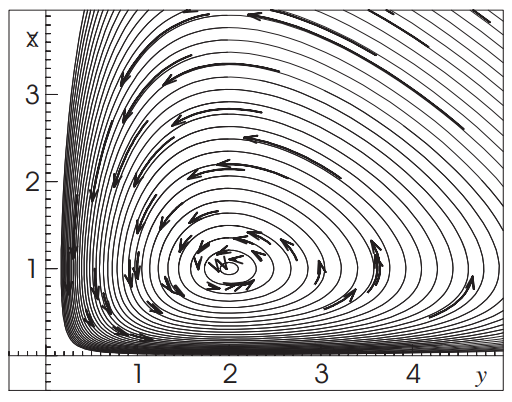
\includegraphics[width=10cm]{snake.png}
						\caption{\textit{Nghiêm của phương trình khi $\alpha = \beta = \gamma = 1, \delta = 2$}}
					\end{center}
				\end{figure*}
			\subsubsection{Chuyển động của 2 vật bởi lực hấp dẫn}
				Xét 2 vật ), K có khối lượng lần lượt là $m_0$, $m_K$. Vật O bị gắn chặt (cố định) tại gốc tọa độ Ox. Điểm K ban đầu cách O một đoạn $x_K > 0$, với vận tốc ban đầu $v_K = 0$. Ta có hệ PTVP mô tả tọa độ của k trong khoảng trục dương của Ox và vận tốc $v$ tương ứng.
				$\left\{\begin{array}{l}
					\frac{dx}{dt} = v \\
					F = ma \Rightarrow -G\dfrac{m_0m_K}{x^2} = m_K\dfrac{dv}{dt}
				\end{array}\right.$ 
				$\Rightarrow \left\{\begin{array}{l}
					\frac{dx}{dt} = v \\
					\frac{dv}{dt} =  -G\frac{m_0}{x^2}
				\end{array}\right.$ \\ \\
				$\Rightarrow \frac{dv}{dt} =  -G\frac{m_0}{x^2v}$ 
				$\Rightarrow vdv = -G\frac{m_0}{x^2}dx$ \\ \\
				$\displaystyle \int_{v_0}^v V\ dV = \displaystyle \int_{x_0}^x -G\frac{m_0}{X^2}\ dX$ \\ \\
				$\Rightarrow \frac{v^2}{2} - \frac{v_0^2}{2} = Gm_0(\frac{1}{x} - \frac{1}{x_0})$ 
				$\Rightarrow v = -\sqrt{2Gm_0}(\frac{1}{x} - \frac{1}{x_0})$
		\subsection{Giải thuật Explicit Euler và Runge Kutta bậc 4}
			\subsubsection{ Euler Explicit}
				Trong toán học và khoa học máy tính, phương pháp Euler là một phương pháp số bậc một để giải các phương trình vi phân thường (ODEs) với giá trị ban đầu cho trước. Nó là phương pháp hiện (explicit) cơ bản nhất cho việc tính tích phân số của các phương trình vi phân thường và là phương pháp Runge-Kutta đơn giản nhất.\\
				Phương pháp Euler là một phương pháp bậc một, có nghĩa là sai số cục bộ (sai số mỗi bước) tỷ lệ thuận với bình phương của kích thước bước, và sai số tổng thể (sai số tại một thời điểm nào đó) tỷ lệ thuận với kích thước bước. Phương pháp Euler thường phục vụ như là cơ sở để xây dựng các phương pháp phức tạp hơn, ví dụ như, phương pháp Dự đoán- Hiệu chỉnh. \\
				Xem xét bài toán tính toán hình dạng của một đường cong chưa biết bắt đầu tại một điểm cho trước và thỏa mãn một phương trình vi phân nào đó. Ở đây, phương trình vi phân có thể được coi như là một công thức mà nhờ nó độ dốc của đường tiếp tuyến với đường cong có thể được tính toán tại điểm bất kỳ nào trên đường cong, một khi vị trí của điểm đó đã được tính toán. \\
				Ý tưởng là trong khi đường cong ban đầu chưa biết, điểm khởi đầu của nó được biểu thị bởi $\displaystyle A_{0}$, là đã biết (xem hình phía trên bên phải). Thì, từ phương trình vi phân, độ dốc của đường cong tại $\displaystyle A_{0}$ có thể được tính toán, và vì vậy, có thể tìm được đường tiếp tuyến.\\
				Đi một bước nhỏ dọc theo đường tiếp tuyến đến một điểm $\displaystyle A_{1}$. Dọc bước nhỏ này, độ dốc không thay đổi quá nhiều, vì vậy $\displaystyle A_{1}$ gần với đường cong.\\
				Phương trình vi phân bậc nhất:
				\begin{center}
					$\left\{\begin{array}{l}
						\dot{x} = f(t,x), \\
						x(t_0) = x_0
					\end{array}\right.$ 
				\end{center}
				Phân tích Taylor:
				\begin{align*}
						x(t+h) &= x(t) + \dot{x}(t) + O(h^2), \\
						&= x(t) + f(t,x(t))h + O(h^2)
				\end{align*}
				Công thức Euler tiến:
				\begin{align*}
					&x_{n+1} = x_n + f(t_n,x_n)h, \\
					Where:\ &x_n := x(t_n) \qquad n = 0,1,2,...
				\end{align*}
				\begin{figure*}[h!]
					\begin{center}
						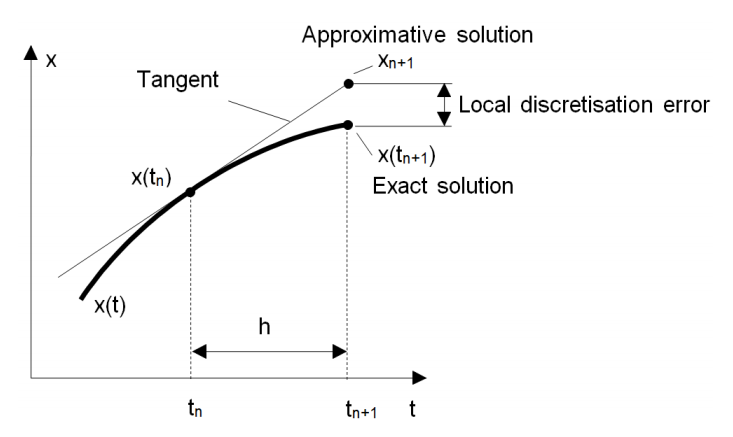
\includegraphics[width=10cm]{euler.png}
						\caption{\textit{Ý nghĩa hình học của Euler tiến}}
					\end{center}
				\end{figure*}
				Nếu chúng ta coi $\displaystyle A_{1}$ vẫn còn nằm trên đường cong, cùng một lý luận như đối với điểm $\displaystyle A_{0}$ có thể tính được độ dốc và tiếp tuyến của đường cong tại $\displaystyle A_{1}$. Sau vài bước, một đường cong đa giác $\displaystyle A_{0}A_{1}A_{2}A_{3}\dots$ được tìm ra. Nói chung, đường cong này không phân kỳ quá xa khỏi đường cong chưa biết ban đầu, và sai số giữa hai đường cong có thể được làm nhỏ nếu kích thước bước là đủ nhỏ và khoảng thời gian tính toán là hữu hạn.
			\subsubsection{Runge Kutta bậc 4 Explicit}
				Trong giải tích số, các phương pháp Runge-Kutta là một họ của các phương pháp lặp ẩn (implicit) và hiện (explicit), trong đó bao gồm thường trình nổi tiếng được gọi là các phương pháp Euler, được sử dụng trong việc rời rạc hóa thời gian để tìm lời giải gần đúng cho các phương trình vi phân thường. \\
				Thành viên được biết đến rộng rãi nhất của họ Runge-Kutta là "RK4", "phương pháp Runge-Kutta cổ điển" hoặc đơn giản là "phương pháp Runge-Kutta". \\
				\textit{Phương pháp Explicit Runge Kutta bậc 4:} Gồm 5 bước tính toán \\
					\underline{Bước 1:} Tính toán độ dốc tại $x_n$
						\begin{align*}
							k_1 = f(t_n, x_n)
						\end{align*}
					\underline{Bước 2:} tính toán độ dốc tại điểm giữa từ $k_1$
						\begin{align*}
							k_2 = f(t_n + \frac{1}{2}h, x_n + \frac{1}{2}hk_1)
						\end{align*}
					\underline{Bước 3:} tính toán độ dốc tại điểm giữa từ $k_2$
						\begin{align*}
							k_3 = f(t_n + \frac{1}{2}h, x_n + \frac{1}{2}hk_2)
						\end{align*}
					\underline{Bước 4:} tính toán độ dốc tại điểm cuối từ $k_2$
						\begin{align*}
							k_4 = f(t_n + h, x_n + hk_2)
						\end{align*}
					\underline{Bước 5:} Tính $x_{n+1}$
						\begin{align*}
							x_{n+1} = x_n + \frac{h}{6}(k_1 + 2k_2 + 2k_3 + k_4)
						\end{align*}
				\begin{figure*}[h!]
					\begin{center}
						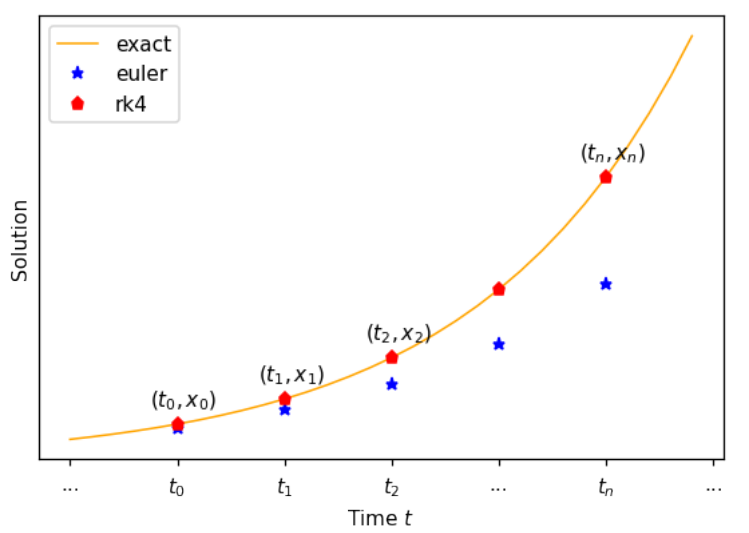
\includegraphics[width=10cm]{kutta.png}
						\caption{\textit{Chuyển tiếp Euler và Runge Kutta bậc 4}}
					\end{center}
				\end{figure*}
		\subsection{Hiện thực hai ví dụ ở phần 2.3 bằng Euler Explicit và Runge Kutta bậc 4 Explicit}
			\subsubsection{Bài toán rắn săn mồi}
				Ta có thể diễn tả bài toán qua hệ động lực dưới đây:
				\begin{align*}
					y' &= y(\alpha - \beta x) \\
					x' &= x(\gamma y - \delta)
				\end{align*}
				Khi $\alpha = \beta = \gamma = 1, \delta = 2$, ta được hệ dưới đây:
				\begin{align*}
					y' &= y(1 - x) \\
					x' &= x(y - 2)
				\end{align*}
				\textbf{\underline{$\bullet$ Phương pháp Euler Explicit:}} \\
					Giả sử tại $t_0$, $x = y = 2$ và h = 0.5, ta có:
					\begin{figure*}[h!]
						\begin{center}
							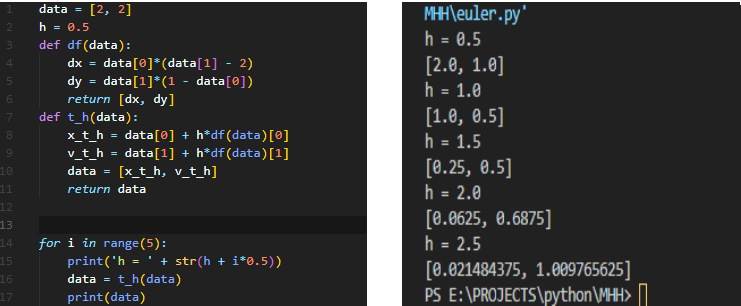
\includegraphics[width=10cm]{snake_euler.png}
							\caption{\textit{Sử dụng Euler Explicit bằng Python để hiện thực bài toán}}
						\end{center}
					\end{figure*}
				\\
				\textbf{\underline{$\bullet$ Phương pháp Runge Kutta bậc 4 Explicit:}} \\
				Giả sử tại $t_0$, $x = y = 2$ và h = 0.5, ta có:
				\begin{figure*}[h!]
					\begin{center}
						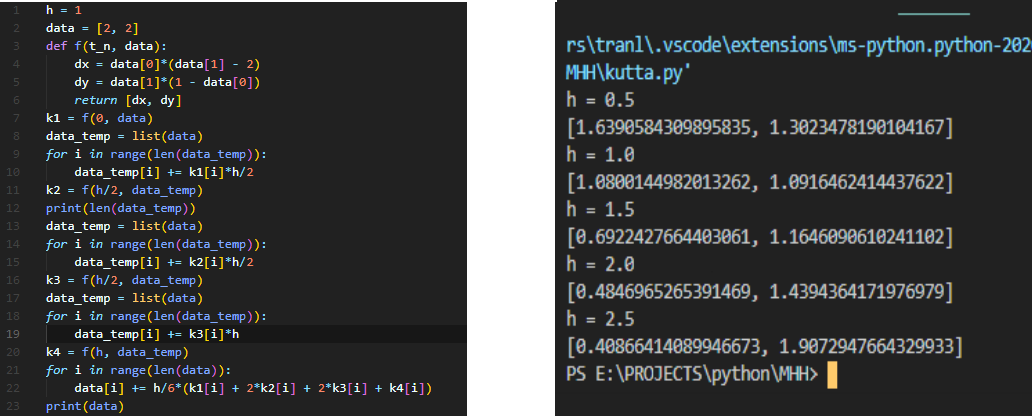
\includegraphics[width=10cm]{snake_kutta.png}
						\caption{\textit{Sử dụng RK4 Explicit bằng Python để hiện thực bài toán}}
					\end{center}
				\end{figure*}
			\subsubsection{Bài toán chuyển động của 2 vật bởi lực hấp dẫn}
				Ta có thể diễn tả bài toán qua hệ động lực dưới đây:
				\begin{align*}
					x' &= v \\
					v' &= -G\frac{m_0}{x^2}
				\end{align*}
				\textbf{\underline{$\bullet$ Phương pháp Euler Explicit:}} \\
					Giả sử tại $m_0 = 1$ và $h = 1$, ta có:
					\begin{figure*}[h!]
						\begin{center}
							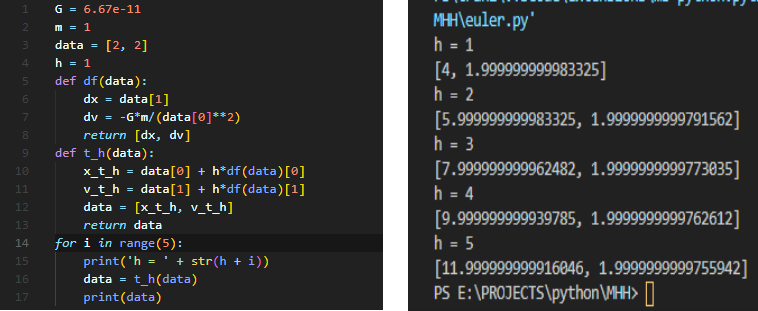
\includegraphics[width=10cm]{vd2_euler.png}
							\caption{\textit{Sử dụng Euler Explicit bằng Python để hiện thực bài toán}}
						\end{center}
					\end{figure*}
				\\
				\textbf{\underline{$\bullet$ Phương pháp Runge Kutta bậc 4 Explicit:}} \\
					Giả sử tại $m_0 = 1$ và $h = 1$, ta có:
					\begin{figure*}[h!]
						\begin{center}
							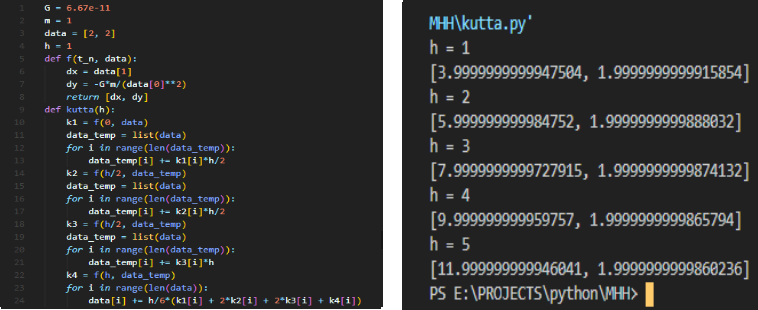
\includegraphics[width=10cm]{vd2_kutta.png}
							\caption{\textit{Sử dụng RK4 Explicit bằng Python để hiện thực bài toán}}
						\end{center}
					\end{figure*}
	\section{Bài 2: Mô hình hệ động lực đối với nồng độ khí \co2 trong nhà kính}						
		\subsection{Sự trao đổi khí \co2}
			Để tổng quát hóa bài toán để có thể áp dụng mô hình trong thực tế, mô hình nhà kính với màn
			chắn nhiệt (thermal screen) được xét trong đề tài này. Màn chắn nhiệt hay còn gọi là tấm chắn
			nhiệt được làm từ nhiều loại vật liệu khác nhau như kim loại hoặc nhựa dẻo có tính đàn hồi.
			Màn chắn nhiệt được sử dụng để bảo vệ cây trồng khỏi thiệt hại gây ra bởi ánh nắng trực tiếp
			từ mặt trời cũng như chống rét cho cây trồng vào mùa đông ở những nơi có khí hậu ôn đới.
			\begin{figure}[h!]
				\begin{center}
					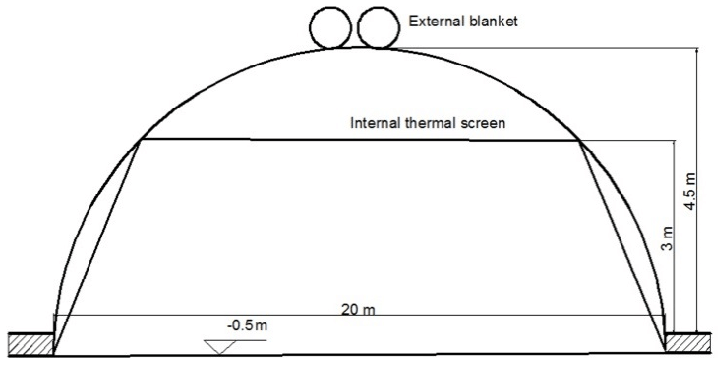
\includegraphics[width=10cm]{thermal_screen.png}
					\caption{\textit{Màn chắn nhiệt có tác dụng che chắn cho cây, điều hòa tiểu khí hậu}}
					\label{h2}
				\end{center}
			\end{figure}
			Màn chắn nhiệt chia nhà kính thành hai gian khác nhau gồm gian nhà kính dưới màn chắn nhiệt và gian nhà kính phía trên màn chắn nhiệt. Vì gian trên thường hẹp hơn gian dưới nhà kính (xem Hình \ref{h2}) nên dẫn đến nồng độ khí \co2 trong không khí ở gian trên và gian dưới nhà kính cũng khác nhau. Sơ đồ tóm tắt sự lưu thông của lượng khí \co2 trong nhà kính khi đó được thể hiện ở Hình \ref{h3}.\\
			Đối với gian dưới của nhà kính, lượng khí \co2 chủ yếu được đưa vào từ các nguồn như luồng gió tự nhiên thông qua hệ thống thông gió và thoát ra ngoài bởi hệ thống quạt (xem Hình \ref{h4} và Hình \ref{h5}). Ngoài ra, lượng khí \co2 ở gian này cũng nhận được bởi các máy sưởi không khí (xem Hình \ref{h6}) trong quá trình đốt nóng tạo nhiệt lượng và bởi bên thứ ba chuyên cung cấp khí \co2. Một phần lượng khí \co2 ở gian dưới nhà kính cũng thất thoát lên gian trên nhà kính dưới sự	điều hướng của sự chênh lệch nhiệt độ và mật độ không khí giữa hai gian cũng như một lượng lớn khí \co2 cũng sẽ được hấp thụ vào trong cây trồng để thực hiện quá trình quang hợp. Đối với gian trên của nhà kính, lượng khí \co2 chủ yếu nhận từ sự trao đổi \co2 với gian dưới và có thể thoát ra bên ngoài thông qua các ô thông gió ở trên mái nhà kính (nếu có) như ở Hình \ref{h9}.
			\begin{figure}[h!]
				\begin{center}
					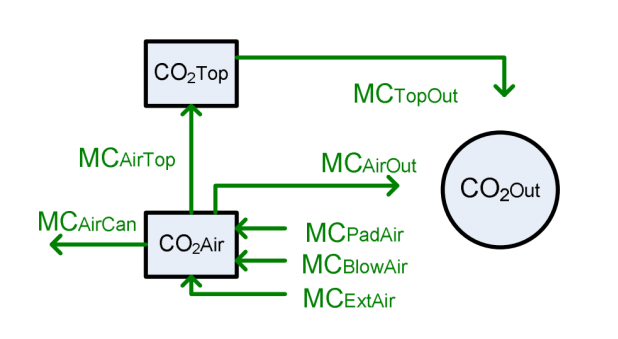
\includegraphics[width=10cm]{co2_flow.png}
					\caption{\textit{Dòng chuyển động của khí \co2 bên trong và bên ngoài nhà kính}}
					\label{h3}
				\end{center}
			\end{figure}
		\subsection{Mô hình Hệ động lực và giả thiết}
			Dựa trên sơ đồ quan sát được ở Hình \ref{h3}, sự thay đổi của nồng độ khí \co2 ở gian dưới và gian trên bên trong nhà kính được biểu diễn qua hệ gồm hai phương trình sau đây. 
			\begin{align}
				\color{blue}
					cap_{\co2_{Air}}\dot{\co2_{Air}} = MC_{BlowAir} +& \textcolor{blue}{MC_{ExAir} + MC_{PadAir}} \nonumber \\ 
					\textcolor{blue}{-}& \textcolor{blue}{MC_{AirCan} - MC_{AirTop} - MC_{AirOut} ,}
					\label{ct1} \\
					\textcolor{blue}{cap_{\co2_{Top}}\dot{\co2_{Top}} = MC_{AirTop} -}& \textcolor{blue}{MC_{TopOut}.}
					\label{ct2}
				\color{blue}
			\end{align}
		
			\begin{figure}[h!]
				\begin{center}
					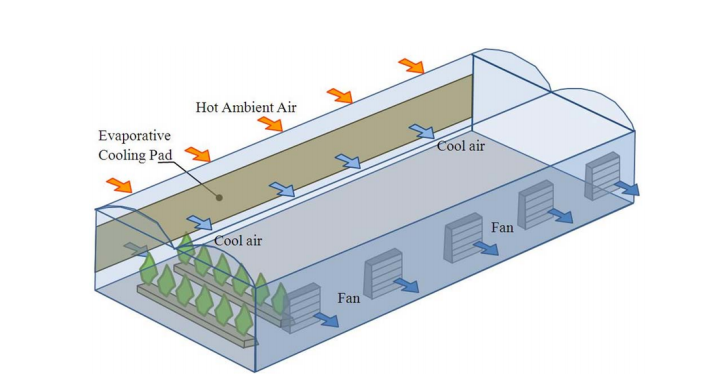
\includegraphics[width=10cm]{co2_line.png}
					\caption{\textit{Dòng chuyển động của khí \co2 thông qua hệ thống gió và quạt}}
					\label{h4}
					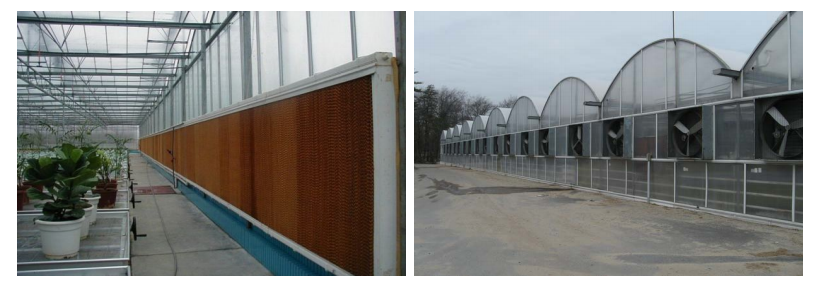
\includegraphics[width=10cm]{vent.png}
					\caption{\textit{Hệ thống gió (trái) và quạt (phải)}}
					\label{h5}
					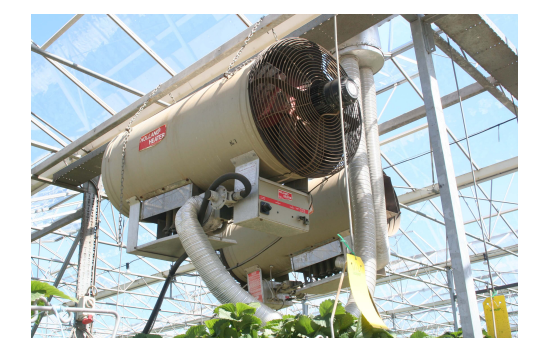
\includegraphics[width=10cm]{heal.png}
					\caption{\textit{Hệ thống sưởi}}
					\label{h6}
				\end{center}
			\end{figure}
			Trong hệ phương trình vi phân này, một số giả thiết đã được xét đến như lượng khí \co2 trong không khí ở gian dưới và trên của nhà kính không bị ảnh hưởng bởi nguồn nào khác ngoại trừ những nguồn đã được thể hiện trong sơ đồ ở hình \ref{h3}. Hơn nữa, nhà kính là một môi trường hoàn hảo theo nghĩa nồng độ \co2 là phân bố đều nhau ở gian dưới và ở gian trên. Các kí hiệu \textit{\textcolor{blue}{$cap_A$}}, \textcolor{blue}{$\co2_A$}, \textcolor{blue}{$\dot{\co2}_A$} và \textit{\textcolor{blue}{$MC_AB$}} lần lượt là khả năng chứa khí \co2 trong \textcolor{blue}{A} (m), nồng độ khí \co2 trong \textcolor{blue}{A} $(mg\ m^{-3})$, tốc độ thay đổi nồng độ khí \co2 trong \textcolor{blue}{A} $(mg\ m^{-3}\ s^{-1})$ và lưu lượng khí \co2 đi từ \textcolor{blue}{A} vào \textcolor{blue}{B} $(mg\ m^{-2}\ s^{-1})$, trong đó \textcolor{blue}{Air} và \textcolor{blue}{Top} đại diện cho gian dưới và gian trên, \textcolor{blue}{Blow} đại diện cho máy sưởi, \textcolor{blue}{Ext} đại diện cho bên thứ ba cung cấp khí \co2, \textcolor{blue}{Pad} đại diện cho hệ thống thông gió, \textcolor{blue}{Can} đại diện cho tán lá cây trồng và \textcolor{blue}{Out} đại diện cho không gian bên ngoài nhà kính. \\
			Dưới đây là source code Python dùng để tính hệ động lực đã được mô tả ở trên:
			
\begin{lstlisting}
# Caculating the differential of Co2 Air and Co2 Top
# ====> return array includes 2 elements [dx_Co2Air, dx_Co2Top]
def derivative(CO2_Air, CO2_Top):
	global temp
	temp -= 1
	mc_air_top = MC_AirTop(CO2_Air, CO2_Top)
	dCO2Air = (MC_BlowAir() + MC_ExtAir() + MC_PadAir(CO2_Air)
			   - MC_AirCan(CO2_Air) - mc_air_top - MC_AirOut(CO2_Air)) / CAP_Co2Air
	dCO2Top = (mc_air_top - MC_TopOut(CO2_Top)) / CAP_Co2Top
	return [dCO2Air, dCO2Top]
\end{lstlisting}
			Hàm \textit{derivative()} nhận vào hai đối số là giá trị của $\co2_{Air}$ và $\co2_{Top}$ tại thời điểm $t$, hàm sẽ tính đạo hàm của nồng độ khí \co2 ở gian dưới \textbf{dCO2Air} và gian trên bên trong nhà kính \textbf{dCO2Top} và trả về một list bao gồm hai giá trị đạo hàm vừa tính được.
			
		\subsection{Phân tích các thông số của hệ động lực}
			Hệ động lực dùng để tính toán sự thay đổi khí \co2 trong nhà kính phụ thuộc vào các công thức \textit{\textcolor{blue}{$MC_AB$}}. \\
			Trước hết, xét lượng \co2 đi từ máy sưởi vào trong gian dưới nhà kính như công thức sau.
			\begin{align}
				\color{blue}
					MC_{BlowAir} = \frac{\eta_{Heat\co2}U_{Blow}P_{Blow}}{A_{Flr}} 
					\tag{3} \label{ct3}
				\color{blue}
			\end{align}
			Trong đó, \textcolor{blue}{$\eta_{Heat\co2}$} là lượng khí \co2 sinh ra khi 1 Joule nhiệt lượng (cảm nhận được) được sinh ra bởi máy sưởi $(mg\ \{\co2\}\ J^{-1})$. Tham số \textcolor{blue}{$U_{Blow}$} thể hiện mức cho phép lượng khí \co2 sinh ra bởi máy sưởi đi vào nhà kính có thể điều chỉnh được trong khoảng \textcolor{blue}{[0, 1]} và không có đơn vị. Hệ số \textcolor{blue}{$P_{Blow}$} là khả năng sinh ra \co2 của máy sưởi (W) và \textcolor{blue}{$A_{Flr}$} là diện tích nhà kính $(m^2)$. \\
			Dưới đây là source code Python dùng để tính $MC_{BlowAir}$: 
\begin{lstlisting}
'''Calculate MC BlowAir'''
# Luong co2 di tu may suoi vao ben trong gian duoi nha kinh
def MC_BlowAir():
	blow_air = (eta_heatCO2 * U_Blow * P_Blow) / A_Flr
	return blow_air
\end{lstlisting}
			Hàm \textit{MC$\_$BlowAir()} sẽ tính giá trị của $MC_{BlowAir}$ dựa trên các tham số đã được xác định, từ đó trả về kết quả. \\ \\
			Tương tự, lượng khí \co2 được bơm vào nhà kính bởi bên thứ ba chuyên cung cấp khí \co2 được cho bởi công thức sau.
			\begin{align}
				\color{blue}
					MC_{ExtAir} = \frac{U_{Ext\co2}\phi_{Ext\co2}}{A_{Flr}} 
				\color{blue}
				\tag{4} \label{ct4}
			\end{align}
			Các kí hiệu \textcolor{blue}{$U_{Ext\co2}$} và \textcolor{blue}{$\phi_{Ext\co2}$} lần lượt là tham số điều chỉnh tốc độ bơm khí \co2 vào trong nhà kính (không có đơn vị) và khả năng bơm \co2 của bên thứ ba $(mg\ s^{-1})$.\\
			Đây là phần hiện thực của công thức trên:
\begin{lstlisting}
'''Calculate MC_ExtAir'''
# Luong khi CO2 duoc bom vao nha kinh boi ben thu ba chuyen cung cap khi CO2
def MC_ExtAir():
	ext_air = (U_Ext * fi_Ext) / A_Flr
	if temp == 0: 
		MC_ExtAirData.append(ext_air)
	return ext_air
\end{lstlisting}
			Hàm \textit{MC$\_$ExtAir()} nhận các tham số tương ứng đã xác định từ trước và trẻ về giá trị của $MC_{ExtAir}$. \\ \\
			
			Mặt khác, lượng khí \co2 đi vào nhà kính thông qua hệ thống thông gió dựa trên sự chênh	lệch của nồng độ khí \co2 bên trong và bên ngoài nhà kính và khả năng cho dòng không khí đi qua của tấm thông gió như hình \ref{h5}. Hơn nữa, khả năng cho dòng không khí đi qua của tấm thông gió có thể điều chỉnh được. Công thức sau dùng để tính \textcolor{blue}{$MC_{PadAir}$}.
			\begin{align}
				\color{blue}
				MC_{PadAir} = f_{Pad}(\co2_{Out} - \co2_{Air}) = \frac{U_{Pad}\phi_{Pad}}{A_{Flr}}(\co2_{Out} - \co2_{Air}) \tag{5} \label{ct5}
				\color{blue}
			\end{align}
			Tốc độ của đi qua tấm thông gió \textcolor{blue}{$f_{Pad}$} $(m\ s^{-1})$ được tính bởi tích của tham số \textcolor{blue}{$U_{Pad}$}, thể hiện mức cho phép lượng khí \co2 đi qua tấm thông gió điều chỉnh được trong khoảng \textcolor{blue}{[0, 1]} và không	có đơn vị, và \textcolor{blue}{$\phi_{Pad}$}, là khả năng cho phép khí \co2 đi qua của tấm thông gió $(m^3\ s^{-1})$ chia cho diện tích nhà kính. \\
			Dưới đây là phần hiện thực phương trình $MC_{PadAir}$:
\begin{lstlisting}
'''Calculate CO2_PadAir'''
# Luong khi CO2 di vao nha kinh thong qua he thong thong gio
def MC_PadAir(CO2_Air):
	f_Pad = U_Pad * fi_Pad / A_Flr     # Toc do CO2 di qua tam thong gio (m^3 s^{-1})
	pad_air = f_Pad*(CO2_Out - CO2_Air)
	return pad_air
\end{lstlisting}
			Hàm \textit{MC$\_$PadAir()} nhận vào đối số là giá trị của $\co2_{Air}$ tại thời điểm t, hàm sẽ tính toán giá trị của $f_{Pad}$, sau đó tính và trả về giá trị $MC_{PadAir}$ dựa vào giá trị của $f_{Pad}$ vừa tính được và các tham số khác đã được xác định. \\ \\
			Đối với lượng khí \co2 đi từ gian dưới lên gian trên nhà kính phức tạp hơn và phụ thuộc vào độ chênh lệch nhiệt độ và độ chênh lệch mật độ của hai gian nhà kính thông qua màn chắn nhiệt.
			\begin{align}
				\color{blue}
					MC_{AirTop} = f_{ThScr}(\co2_{Air} - \co2_{Top}) \tag{6} \label{ct6}
				\color{blue}
			\end{align}
			trong đó tốc độ lưu thông khí \co2 qua màn chắn nhiệt \textcolor{blue}{$f_{ThScr}$} $(m\ s^{-1})$ là tổng của hai tốc độ gồm tốc độ thẩm thấu qua màn chắn nhiệt và tốc độ tại những nơi không bị chắn bởi màn chắn nhiệt (xem Hình \ref{h7}).
			\begin{align}
				\color{blue}
					f_{ThScr} = U_{ThScr}K_{ThScr}{\vert T_{Air} - T_{Top} \vert}^{\frac{2}{3}} + (1 - U_{ThScr}) \left[\frac{g(1 - U_{ThScr})}{2\rho^{Mean}_{Air}}\vert\rho_{Air} - \rho_{Top}\vert\right]^{\frac{1}{2}}
	   			\tag{7} \label{ct7}
				\color{blue}
			\end{align}
			Ở những nơi có màn chắn nhiệt với độ phủ \textcolor{blue}{$U_{ThScr} \in [0, 1]$} (không có đơn vị), tốc độ phụ thuộc
			\begin{figure}[h!]
				\begin{center}
					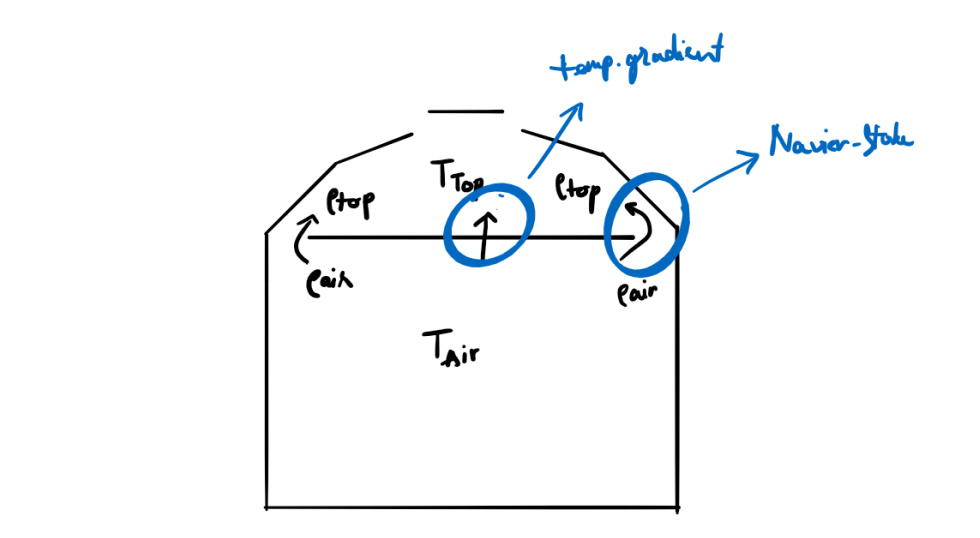
\includegraphics[width=10cm]{co2_move.png}
					\caption{\textit{Chuyển động của khí \co2 qua mzàn chắn nhiệt}}
					\label{h7}
				\end{center}
			\end{figure}
			vào sự chênh lệch giữa nhiệt độ bên trên \textcolor{blue}{$T_{Top}$} (K) và bên dưới \textcolor{blue}{$T_{Air}$} (K) màn chắn và khả năng cho không khí thẩm thấu của màn chắn là \textcolor{blue}{$K_{ThScr}$} $(m\ K^{-\frac{2}{3}}\ s^{-1})$. Ở những nơi không có màn chắn nhiệt với độ phủ \textcolor{blue}{$1 - U_{ThScr}$}, tốc độ được cho bởi một phương trình Navier–Stokes phụ thuộc vào sự chênh lệch của mật độ không khí \textcolor{blue}{$T\rho_{Air}$} và \textcolor{blue}{$T\rho_{Top}$} cùng tính bằng đơn vị $(kg\ m^{-3})$. Hệ số \textcolor{blue}{$\dfrac{2}{3}$} trong công thức (\ref{ct7}) đến từ thực nghiệm trong công trình của [Bal89]. Trong công trình đó, tác giả đã sử dụng dữ liệu đo đạc được về tốc độ trao đổi không khí thông qua	các màn chắn làm từ 12 loại chất liệu khác nhau và sử dụng chúng để huấn luyện mô hình \textcolor{blue}{$K_{ThScr}{\vert T_{Air} - T_{Top} \vert}^m$} với \textcolor{blue}{m} là tham số điều chỉnh được để tìm ra \textcolor{blue}{m} gần bằng \textcolor{blue}{$0.66$} là \textcolor{blue}{$\dfrac{2}{3}$}.\\
			Hàm mô tả tính toán $MC_{AirTop}$ và các tham số của hàm được thể hiện dưới đây:
\begin{lstlisting}
# Toc do luu thong khi CO2 qua man chan nhiet
def f_ThScr():
	# Mat do khong khi duoi man chan nhiet (kg m^{-3})
	p_Air = p_Air0 * math.exp(g * M_Air * h_Elevation / (T_Air * R * 1000))  
	# Mat do khong khi tren man chan nhiet (kg m^{-3})
	p_Top = p_Air0 * math.exp(g * M_Air *(h_Elevation + h_Air) / (T_Top * R * 1000))  
	# Mat do khong khi trung binh
	p_MeanAir = p_Air0 * math.exp(g * M_Air*(h_Elevation + h_Gh) / ((T_Air + T_Top)/2 * R * 1000))
	
	thScr       = U_ThScr * K_ThScr * (abs(T_Air - T_Top)) ** (2/3)
	notThScr    = (1 - U_ThScr) * ( g*(1 - U_ThScr) / (2*p_MeanAir) * abs(p_Air - p_Top) )**0.5
	return thScr + notThScr
	
# Luong khi CO2 di tu gian duoi len tren nha kinh
def MC_AirTop(CO2_Air, CO2_Top):
	air_top = f_ThScr() * (CO2_Air - CO2_Top)
	if temp == 0: 
		MC_AirTopData.append(air_top)
	return air_top
\end{lstlisting}
			Hàm \textit{f$\_$ThScr()} dùng để tính và trả về giá trị của $f_{ThScr}$ bằng cách tính tổng của hai tốc độ gồm tốc độ thẩm thấu qua màn chắn nhiệt (biến \textbf{thScr}) và tốc độ tại những nơi không bị chắn bởi màn chắn nhiệt(biến \textbf{notThScr}). Dựa vào kết quả của hàm  \textit{f$\_$ThScr()}, giá trị của $\co2_{Air}$ và $\co2_{Top}$ tại thời điểm $t$ và các giá trị tham số xác định khác, hàm \textit{MC$\_$AirTop()} sẽ tính ra giá trị của $MC_{AirTop}$ và trả về kết quả tương ứng. \\ \\
			 
			Tương tự, để biểu diễn lượng khí \co2 từ bên trong ra bên ngoài nhà kính theo hai hướng từ gian dưới và từ gian trên qua các ô thông gió ta sử dụng các công thức như dưới đây.
			\begin{align}
				\color{blue}
					MC_{AirOut} = (f_{VentSide} + f_{VentForced})(\co2_{Air} - \co2_{Out})
					\tag{8} \label{ct8}
				\color{blue}
			\end{align}
			Trong đó, \textcolor{blue}{$f_{VentSide}$} là tốc độ gió của hệ thống quạt trên tường bao xung quanh nhà kính và \textcolor{blue}{$f_{VentForced}$} là tốc độ gió từ hệ thống quạt bên trong nhà kính, cả hai tốc độ đều được đo với đơn vị $(m\ s^{-1})$. Tuy nhiên trong trường hợp này, nguyên lý Bernouilli đóng vai trò quan trọng biểu diễn bởi độ chênh lệch áp suất từ phía ngoài nhà kính gây ra bởi luồng gió tự nhiên và áp suất từ phía trong nhà kính gây ra do luồng không khí bên trong (xem Hình \ref{h8}), hiệu ứng Stack hay còn gọi là hiệu ứng Chimney cũng cần được xét đến (xem Hình \ref{h9}). Hiệu ứng Stack là hiệu ứng mà vào mùa đông, dòng không khí lạnh từ bên ngoài vào bên trong nhà kính và bị làm nóng dần bởi hệ thống sưởi và có xu hướng đi lên phía trên mái nhà kính và thoát ra trở lại bên ngoài, vào mùa hè thì theo chiều ngược lại.
			\begin{figure}[h!]
				\begin{center}
					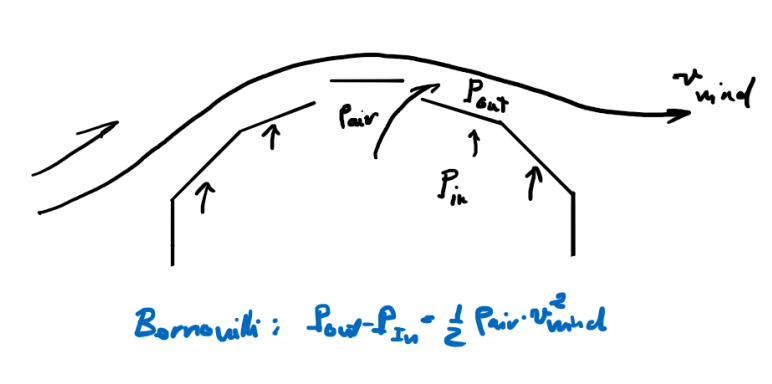
\includegraphics[width=10cm]{flow_roof_open.png}
					\caption{\textit{Dòng không khí qua ô mở mái nhà kính}}
					\label{h8}
				\end{center}
			\end{figure}
			\\
			Để tổng quát hóa mô hình cho nhiều loại nhà kính khác nhau, công thức tổng quát dưới đây \textcolor{blue}{$f_{VentRoofSide}$} $(m s^{-1})$ được dùng để thiết lập công thức cho \textcolor{blue}{$f_{VentSide}$}.
			\begin{align}
				\textcolor{blue}{f_{VentRoofSide} = \frac{C_d}{A_Flr}\left[\frac{U^2_{Roof}U^2_{Side}A^2_{Roof}A^2_{Side}}{U^2_{Roof}A^2_{Roof} + U^2_{Side}A^2_{Side}}\cdot \frac{2gh_{SideRoof}(T_{Air} - T_{Out})}{T^{Mean}_{Air}}\right.} \nonumber \\
				\textcolor{blue}{\left. + (\frac{U_{Roof}A_{Roof} + U_{Side}A_{Side}}{2})^2C_{\omega}v^2_{Wind}\right]^{\frac{1}{2}}}
				\tag{9} \label{ct9}
			\end{align}
			\begin{figure}[h!]
				\begin{center}
					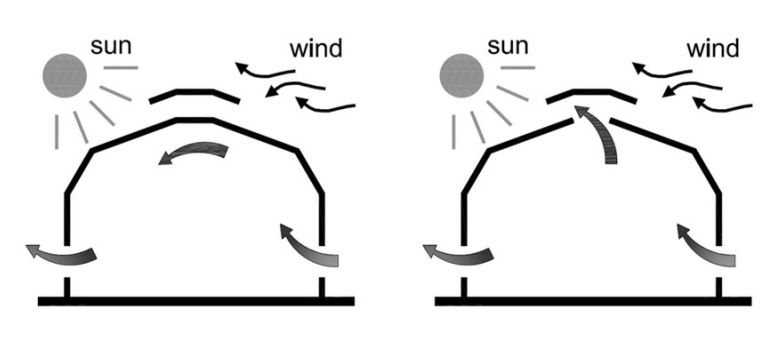
\includegraphics[width=10cm]{chimeny.png}
					\caption{\textit{Không có hiệu ứng Stack (trái) và có hiệu ứng stack (phải)}}
					\label{h9}
				\end{center}
			\end{figure}
			Công thức \eqref{ct10} là tổng của hai thành phần nhân với tỷ lệ giữa hệ số lưu lượng gió \textcolor{blue}{$C_d$} không có đơn vị và diện tích nhà kính \textcolor{blue}{$A_{Flr}$} $(m^2)$. Thành phần thứ nhất phụ thuộc vào độ chênh lệch nhiệt độ giữa bên ngoài và bên trong nhà kính (ở gian dưới màn chắn nhiệt) đại diện cho hiệu ứng Stack khi diện tích ô thông gió trên mái \textcolor{blue}{$A_{Roof}$} $(m^2)$ là khác không. Thành phần thứ hai cho bởi độ chênh lệch áp suất bên trong và bên ngoài nhà kính và được tính bằng tổng diện tích các nơi thông gió trên nhà kính chia hai nhân vận tốc gió tự nhiên \textcolor{blue}{$v_{Wind}$} $(m\ s^{-1})$ và hệ số áp suất
			gió \textcolor{blue}{$C_w$} không có đơn vị. Các hệ số \textcolor{blue}{$Cd$} và \textcolor{blue}{$C_w$} là các hệ số lý thuyết phụ thuộc vào cấu trúc và hình dáng của nhà kính và có thể ước lượng được thông qua các số liệu đo đạc được trên thực nghiệm. \\ \\ \\
			Ngoài ra, lưới chắn côn trùng gây hại trên các nơi thông gió và hệ số rò rỉ của nhà kính cũng sẽ được xét trong đề tài này. Khi có lưới chắn côn trùng, tốc độ chuyển động của các luồng không khí qua các nơi thông gió sẽ giảm xuống với hệ số
			\begin{align}
				\textcolor{blue}{\eta_{InsScr} = \zeta_{InsScr}(2 - \zeta_{InsScr}),}
				\tag{10} \label{ct10}
			\end{align}
			trong đó \textcolor{blue}{$\zeta_{InsScr}$} không có đơn vị là độ rổ của lưới, nghĩa là tỷ lệ diện tích các lỗ trên lưới và tổng diện tích lưới chắn côn trùng. Với hệ số rò rỉ \textcolor{blue}{$c_{leakage}$} không có đơn vị, tốc độ trao đổi không khí thường được xấp xỉ khoảng $50\%$ tốc độ
	
			\begin{align}
				\textcolor{blue}{f_{leakage} = \left\{\begin{array}{rcl}
					0.25\cdot c_{leakage}, & v_{Wind} < 0.25, \\
					v_{Wind}\cdot c_{leakage}, & v_{Wind} \geq 0.25
				\end{array}\right.}
				\tag{11} \label{ct11}
			\end{align}
			Một cách ngầm hiểu, giả thiết về phân bố đều của sự rò rỉ của nhà kính đã được sử dụng. \\
			Gọi \textcolor{blue}{$\eta_{Side\_Thr}$} là ngưỡng Stack, nghĩa là nếu \textcolor{blue}{$\eta_{Side}$} là tỷ lệ giữa diện tích các nơi thông gió trên tường bao quanh nhà kính và diện tích của tất cả các nơi thông gió trên nhà kính và \textcolor{blue}{$\eta_{Side}$} vượt ngưỡng Stack thì hiệu ứng Stack không xảy ra và ngược lại. Khi đó, \textcolor{blue}{$f_{VentSide}$} được cho bởi công thức sau.
			\begin{align}
				\textcolor{blue}{f_{VentSide} = \left\{\begin{array}{lll}
						\eta_{InsScr}f^{''}_{VentSide} + 0.5f_{leakage}, & \eta_{Side} \geq \eta_{Side\_Thr}, \\
						\eta_{InsScr}\left[U_{ThScr}f^{''}_{VentSide}\right.  \\
						+ \left(1 - U_{ThScr})f_{VentRoofSide}\eta_{Side}\right] + 0.5f_{leakage}, & \eta_{Side} < \eta_{Side\_Thr}
					\end{array}\right.}
				\tag{12} \label{ct12}
			\end{align}
			Trong đó, \textcolor{blue}{$f^{''}_{VentSide}$} là \textcolor{blue}{$f_{VentRoofSide}$} tính tại \textcolor{blue}{$A_{Roof} = 0$}. Lưu ý, ở những nơi phủ bởi màn chắn nhiệt, hiệu ứng Stack cũng không xảy ra. \\
			Tốc độ \textcolor{blue}{$f_{VentForced}$} bởi hệ thống quạt gió bên trong nhà kính được tính bởi công thức sau.
	
			\begin{align}
				\color{blue}
					f_{VentForced} = \frac{\eta_{InsScr}U_{VentForced}\phi_{VentForced}}{A_{Flr}}.
				\color{blue}
				\tag{13} \label{ct13}
			\end{align}
			Kí hiệu \textcolor{blue}{$U_{VentForced}$} không có đơn vị thể hiện sự điều chỉnh tốc độ gió mà hệ thống có thể	\textcolor{blue}{$\phi_{VentForced}$} $(m^3\ s^{-1})$ và có giá trị trong khoảng \textcolor{blue}{[0, 1]}. \\
			Phần hiện thực hàm tính $MC_{AirOut}$ và các giá trị liên quan tới nó được thể hiện ở đây:
\begin{lstlisting}
def f_VentRoofSide(A_Roof):
	p1 = (U_Roof*U_Side*A_Roof*A_Side) ** 2
	p2 = (U_Roof * A_Roof) ** 2 + (U_Side * A_Side)**2
	p3 = 2*g*h_Side_Roof*(T_Air - T_Out)/T_Mean
	p4 = ((U_Roof*A_Roof + U_Side*A_Side)/2) ** 2
	
	if A_Roof == 0 and A_Side == 0:
		return 0
	return (cd/A_Flr)*((p1/p2*p3 + p4*cw*(v_wind**2)) ** 0.5)

# toc do gio cua he thong quat tren tuong
def f_VentSide():
    if U_Roof == 0:
		eta_Roof = 1
		eta_Side = 1
	else:
		eta_Roof = A_Roof * U_Roof / (A_Side * U_Side + A_Roof * U_Roof)
		eta_Side = (A_Side * U_Side) / (A_Side * U_Side + A_Roof * U_Roof)
	if eta_Roof < eta_Side_Thr:
		return zeta_InsScr() * (U_ThScr*f_VentRoofSide(0)+(1-U_ThScr) * f_VentRoofSide(A_Roof) *eta_Side) + 0.5*f_Leakage()
	else:
		return zeta_InsScr()*f_VentRoofSide(0)+0.5*f_Leakage()

# He so giam do luoi chan con trung
def zeta_InsScr():
	return zeta_Insect * (2 - zeta_Insect)

# Cuong do khong khi ro ri
def f_Leakage():
	if v_wind < 0.25:
		return 0.25*c_leak
	else:
		return v_wind*c_leak

# toc do boi he thong quat gio trong nha kinh
def f_VentForced():
	return zeta_InsScr()*U_VentForced*fi_VentForced/A_Flr

# Calculate MC_AirOut
def MC_AirOut(CO2_Air):
	air_out = (f_VentSide() + f_VentForced()) * (CO2_Air - CO2_Out)
	if temp == 0:
		MC_AirOutData.append(air_out)
	return air_out
\end{lstlisting}
			Trong các hàm ở trên, hàm  \textit{f$\_$VentRoofSide()} nhận đối số là diện tích của thông gió trên mái, cùng với các giá trị tham số cho trước để tính chính xác và trả về giá trị của $f_{VentRoofSide}$, hàm \textit{zeta$\_$InsScr()} dựa vào giá trị của $\zeta_{InsScr}$ để tính toán và trả về giá trị của $\eta_{InsScr}$, hàm \textit{f$\_$Leakage()} trả về giá trị cường độ không khí rò rỉ $f_{Leakage}$. Giá trị trả về của ba hàm này được sử dụng bởi hàm \textit{f$\_$VentSide()} để tính toán và trả về giá trị của $f_{VentSide}$. Tương tự,  hàm \textit{f$\_$VentForced()} sử dụng giá trị trả về của hàm \textit{zeta$\_$InsScr()} để tính toán ra kết quả của $f_{VentForced}$. Dựa vào kết quả trả về của hai hàm \textit{f$\_$VentSide()} và hàm \textit{f$\_$VentForced()}, giá trị của $MC_{AirOut}$ được tính toán như trong phương trình (\ref{ct8}), cụ thể là được thực hiện thông qua hàm \textit{MC$\_$AirOut()}.\\ \\
			
			Tương tự như \textcolor{blue}{$MC_{AirOut}$}, lượng khí \co2 đi từ gian trên nhà kính ra ngoài thông qua ô mở trên mái nhà kính được tính bởi công thức
			\begin{align}
				\color{blue}
					MC_{TopOut} = f_{VentRoof}(\co2_{Top} - \co2_{Out}).
				\color{blue}
				\tag{14} \label{ct14}
			\end{align}
			Trong đó, \textcolor{blue}{$f_{VentRoof}$} là tốc độ luồng không khí đi qua ô mở mái nhà kính và được cho bởi công thức sau.
			\begin{align}
				\textcolor{blue}{f_{VentRoof} = \left\{\begin{array}{lll}
						\eta_{InsScr}f^{''}_{VentRoof} + 0.5f_{leakage}, & \eta_{Roof} \geq \eta_{Roof\_Thr}, \\
						\eta_{InsScr}\left[U_{ThScr}f^{''}_{VentRoof}\right.  \\
						+ \left(1 - U_{ThScr})f_{VentRoofSide}\eta_{Side}\right] + 0.5f_{leakage}, & \eta_{Roof} < \eta_{Roof\_Thr}
					\end{array}\right.}
				\tag{15} \label{ct15}
			\end{align}
			Tuy nhiên, khác với \textcolor{blue}{$f_{VentSide}$} trong công thức (\ref{ct12}), khi tỷ lệ \textcolor{blue}{$\eta_{Roof}$} giữa diện tích ô mở trên mái nhà kính và tổng diện tích các ô thông gió trên nhà kính vượt ngưỡng Stack là \textcolor{blue}{$\eta_{Roof_Thr}$}, nghĩa
			là hiệu ứng Stack không xảy ra, ta không thể sử dụng công thức \textcolor{blue}{$f_{VentRoofSide}$} trong (\ref{ct9}) với \textcolor{blue}{$A_{Side} = 0$} để tính \textcolor{blue}{$f^{''}_{VentRoof}$} mà phải sử dụng công thức sau 
			\begin{align}
				\color{blue}
				f^{''}_{VentRoof} = \frac{C_dU_{Roof}A_{Roof}}{2A_{Flr}}\left[\frac{gh_{Roof}(T_{Air} - T_{Out})}{2T^{Mean}_{Air}} + C_wv^2_{Wind}\right]^{\frac{1}{2}}.
				\color{blue}
				\tag{16} \label{ct16}
			\end{align}
			Dựa vào các phương trình được mô tả trên, ta có thể hiện thực hàm tính $MC_{TopOut}$ và các giá trị liên quan qua source code python dưới đây:
\begin{lstlisting}
# toc do khong khi di qua o mo mai nha kinh
def f_VentRoof():
	if U_Roof == 0:
		eta_Roof = 1
	else:
		eta_Roof = A_Roof * U_Roof / (A_Side * U_Side + A_Roof * U_Roof)
		
	if eta_Roof < eta_Roof_Thr:
		return zeta_InsScr() * (U_Roof*f2_VentRoof() + (1-U_Roof) * f_VentRoofSide(A_Roof) * eta_Roof)+0.5*f_Leakage()
	else:
		return zeta_InsScr()*f2_VentRoof()+0.5*f_Leakage()

def f2_VentRoof():
	return (cd*U_Roof*A_Roof)/(2*A_Flr) * ((g*h_Vent*(T_Air-T_Out)/(2*T_Mean)+cw*(v_wind**2)) ** 0.5)

'''Calculate MC_TopOut'''
def MC_TopOut(CO2_Top):
	top_out = f_VentRoof()*(CO2_Top - CO2_Out)
	if temp == 0:
		MC_TopOutData.append(top_out)
	return top_out
\end{lstlisting}
			hàm \textit{f2$\_$VentRoof()} nhận vào các giá trị tham số tương ứng để trả về giá trị của $f^{''}_{VentRoof}$. Dựa vào kết quả của hàm này và các hàm  phụ trợ dùng để tính phương trình (\ref{ct8}) đã được giải thích ở trên, ta sẽ tính được giá trị của $f_{VentRoof}$. Cuối cùng là hàm chính dùng để hiện thực $MC_{TopOut}$, hàm này nhận vào 2 đối số là $\co2_{Top}$ và $\co2_{Out}$ tại thời điểm t, kết hợp với giá trị $f_{VentRoof}$ đã được tính ở trên. \\ \\
			
			Cuối cùng, chúng ta cần mô tả lượng khí \co2 bị hấp thụ vào trong tán lá thông qua quá trình quang hợp.
			\begin{align}
				\color{blue}
				MC_{AirCan} = M_{CH_2O}h_{C_{Buf}}(P - R).
				\color{blue}
				\tag{17} \label{ct17}
			\end{align}
			Trong đó \textcolor{blue}{$M_{CH_2O}$} là khối lượng mol \textcolor{blue}{$CH_2O$} $(mg\ \mu mol^{-1})$, \textcolor{blue}{$P$} là tốc độ quang hợp $(\mu mol\ \{\co2\}\ m^{-2}\ s^{-1})$, \textcolor{blue}{$R$} là tốc độ hô hấp của cây $(\mu mol\ \{\co2\}\ m^{-2}\ s^{-1})$ và hệ số
			\begin{align}
				\textcolor{blue}{h_{C_{Buf}} = \left\{\begin{array}{lll}
						0, & C_{Buf} > C^{Max}_{Buf}, \\
						1, & C_{Buf} \leq C^{Max}_{Buf}
					\end{array}\right.}
				\tag{18} \label{ct18}
			\end{align}
			thể hiện sự ngưng quá trình quang hợp khi lượng \textcolor{blue}{$CH_2O$} là \textcolor{blue}{$C_{Buf}$} $(mg\ \{CH_2O\}\ m^{-2})$ sinh ra đã vượt sức chứa của cây \textcolor{blue}{$C^{Max}_{Buf}$} $(mg\ \{CH_2O\}\ m^{-2})$. Thông thường, tốc độ hô hấp của cây không đáng kể so với tốc độ quang hợp của cây và có thể được lược bỏ hoặc được tính vào khoảng $1\%$ của tốc độ quang hợp của cây. \\
			Tốc độ quang hợp ở tán cây $P$ được mô tả bởi
			\begin{align}
				\color{blue}
					P = \dfrac{J \cdot (\co2_{Stom} - \Gamma)}{4(\co2_{Stom} + 2\Gamma)}
				\color{blue}
				\tag{19} \label{ct19}
			\end{align}
			Trong đó, $J\ (\mu mol\ \{e^{-}\}\ m^{-2}s^{-1})$ là tốc độ chuyển động của electron, $4\ (\mu mol\ \{e^{-}\}\ \mu mol^{-1}\ {\co2})$ là số electron trên mỗi phân tử \co2 cố định, $\co2_{Stom}\ (\mu mol\ \{\co2\}\ mol^{-1}\ \{Air\})$ và $\Gamma$ $(\mu mol\ \{\co2\}\ mol^{-1}\ \{Air\})$ là điểm bù \co2.\\
			Tốc độ hô hấp $R$ được mô tả bởi
			\begin{align}
				\color{blue}
					R = P \cdot \dfrac{\Gamma}{\co2_{Stom}}
				\color{blue}
				\tag{20} \label{ct20}
			\end{align}
			Tốc độ vận chuyển electron $J$ được tính bởi
			\begin{align}
				\color{blue}
					J = \dfrac{J^{POT} + \alpha PAR_{Can} - \sqrt{(J^{POT} + \alpha PAR_{Can})^2 - 4\Theta \cdot J^{POT} \cdot \alpha PAR_{Can}}}{2\Theta}
				\color{blue}
				\tag{21} \label{ct21}
			\end{align}
			Trong đó, $J^{POT}\ (\mu mol\ \{e^{-}\}\ m^{-2}\ s^{-1})$ là tốc độ tiềm năng của sự vận chuyển electron, $PAR_{Can}$ $(\mu mol\ \{photons\}\ m^{-2}\ s^{-1})$ là PAR bị thẩm thấu, $\alpha\ (\mu mol\ \{e^{-}\}\ \mu mol^{-1}\ {photons})$ là hệ số chuyển đổi từ photon thành electron và $\Theta\ (-)$ là mức độ cong của tốc độ vận chuyển electron. \\
			Tốc độ tiềm năng của sự vận chuyển electron $J^{POT}$ phụ thuộc vào nhiệt độ
			\begin{align}
				\color{blue}
					J^{POT} = J^{MAX}_{25,Can} \cdot e^{E_j\dfrac{T_{Can,K} - T_{25,K}}{R\cdot T_{Can,K} \cdot T_{25,K}}} \cdot \dfrac{1 + e^{\dfrac{S\cdot T_{25,K} - H}{R\cdot T_{25,K}}}}{1 + e^{\dfrac{S \cdot T_{Can,K} - H}{R\cdot T_{Can,K}}}}
				\color{blue}
				\tag{22} \label{ct22}
			\end{align}
			Trong đó, $J^{MAX}_{25,Can}$ $(\mu mol\ \{e^{-}\}\ m^{-2}\ s^{-1})$ là tốc độ vận chuyển electron tối đa ở $25^oC$ đối với tán cây, $E_j$ $(J\ mol^{-1})$ là năng lượng kích hoạt cho $J^{POT}$, $T_{Can,K}$ $(K)$ là nhiệt độ tán cây, $T_{25,K}$ $(K)$ là nhiệt độ tương quan tại $25^oC$, $R$ $(J\ mol^{-1}\ K^{-1})$ là hằng số khí, $S$ $(J\ mol^{-1}\ K^{-1})$ là hàm trạng thái entropy và $H$ $(J\ mol^{-1}\ K^{-1})$ là năng lượng ngừng kích hoạt. \\
			Tốc độ vận chuyển electron tối đa ở $25^oC$, $J^{MAX}_{25,Can}$  được tính bằng
			\begin{align}
				\color{blue}
					J^{MAX}_{25,Can} = LAI \cdot J^{MAX}_{25,Leaf}
				\color{blue}
				\tag{23} \label{ct23}
			\end{align}
			Trong đó, $J^{MAX}_{25,Leaf}$ $(\mu mol\ \{e^{-}\}\ m^{-2}\ s^{-1})$ là tốc độ vận chuyển electron tối đa trong lá ở $25^oC$, \lai là chỉ số diện tích lá (leaf area index - \lai). \\
			Chỉ số \lai được tính bởi tổng mật độ độ lá trên một đơn vị diện tích đất trong nhà kính. Khi đó, nếu tán lá càng dày thì chỉ số \lai càng cao (xem Hình \ref{h16}).		
			\begin{figure}[h!]
				\begin{center}
					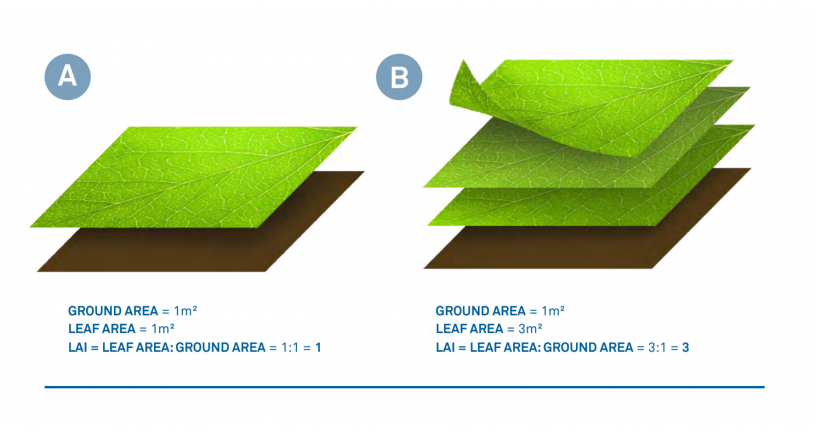
\includegraphics[width=8cm]{lai.png}
					\caption{\textit{Chỉ số diện tích lá}}
					\label{h16}
				\end{center}
			\end{figure} 
			\newpage
			Nồng độ khí \co2 bên trong khí khổng, $\co2_{Stom}$ phụ thuộc vào độ dẫn của khí khổng và mô thực vật, sức cản của lớp ranh giới, tốc độ quang hợp và sự chênh lệch giữa nồng độ CO2 trong khí khổng và nồng độ CO2 của không khí trong nhà kính. Tuy nhiên, nồng độ CO2 trong khí khổng được giả định là một phần cố định của nồng độ CO2 trong nhà kính.
			\begin{align}
				\color{blue}
					\co2_{Stom} = \eta_{\co2 Air\_Stom} \cdot \co2_{Air}
				\color{blue}
				\tag{24} \label{ct24}
			\end{align}
			Trong đó, $\eta_{\co2 Air\_Stom}$ $(-)$ là hệ số chuyển đổi từ nồng độ \co2 trong nhà kính. \\
			Điểm bù \co2 $\Gamma$ ảnh hưởng đến tốc độ quang hợp của lá và phụ thuộc vào nhiệt độ
			\begin{align}
				\color{blue}
					\Gamma = c_{\Gamma}T_{Can}
				\color{blue}
				\tag{25} \label{ct25}
			\end{align}
			Trong đó, $c_{\Gamma}$ $(\mu mol\ \{\co2\}\ mol^{-1}\ \{Air\} K^{-1})$ xác định sự ảnh hưởng của nhiệt độ tán lá đến điểm bù CO2. \\
			Mối quan hệ giữa nhệt độ tán lá và điểm bù \co2 có thể dùng để tính tốc độ quang hợp của lá. Tuy nhiên, áp dụng công thức (\ref{ct25}) với tầng tán lá dẫn đến nhiệt độ tán lá tối ưu thấp không thực tế đối với tốc độ quang hợp khi mức co2 và ánh sáng yếu, bởi vì dựa vào công thức \ref{ct24}, $J^{MAX}_{25,Can}$ lớn hơn so với $J^{MAX}_{25,Leaf}$. Để tránh điều này xảy ra, ta sẽ cho $\Gamma$ phụ thuộc vào tỉ lệ giữa $J^{MAX}_{25,Can}$ và $J^{MAX}_{25,Leaf}$
			\begin{align}
				\color{blue}
					\Gamma = \dfrac{J^{MAX}_{25,Leaf}}{J^{MAX}_{25,Can}}c_{\Gamma}T_{Can} + 20C_{\Gamma} (1 - \dfrac{J^{MAX}_{25,Leaf}}{J^{MAX}_{25,Can}})
				\color{blue}
				\tag{26} \label{ct26}
			\end{align}
			Công thức (\ref{ct26}) được sử dụng để đảm bảo rằng đối với tất cả giá trị của $J^{MAX}_{25,Can}$ ở $20^oC$, điểm bù được tính bằng công thức (\ref{ct26}) sẽ bằng với điểm bù được tính bằng công thức (\ref{ct25}).
			
			Các công thức từ (\ref{ct17})-(\ref{ct26}) được hiện thực qua source code Python sau:
\begin{lstlisting}
# Toc do quang hop
def P(CO2_Air):
	return J()*(CO2_Stom(CO2_Air) - tau()) / (4*(CO2_Stom(CO2_Air) + 2*tau()))

# Toc do ho hap
def R_(CO2_Air):
	return P(CO2_Air) * tau() / CO2_Stom(CO2_Air)

# Nong do co2 trong khi khong
def CO2_Stom(CO2_Air):
	return eta_CO2AirStom * CO2_Air

# Diem bu nong do co2 trong khi khong
def tau():
	T_Can = T_Air + 10
	return cT*T_Can/LAI + 20*cT*(1-1/LAI)

# Toc do truyen e
def J():
	sum = J_POT() + alpha*PAR_Can
	product = J_POT() * alpha*PAR_Can
	return (sum - (sum**2 - 4*theta*product)**0.5) / (2*theta)

# Toc do truyen e tiem nang
def J_POT():
	T_Can = T_Air + 10
	factor1 = math.exp(Ej * (T_Can - T25) / (R * T_Can * T25))
	factor2 = (1 + math.exp((S*T25 - H)/(R*T25))) / \ (1 + math.exp((S*T_Can - H)/(R*T_Can)))
	return J_MAX25Can() * factor1 * factor2

# Toc do truyen e lon nhat o 25'c cua tan la
def J_MAX25Can():
	return LAI * J_MAX25Leaf
	
'''Calculate MC_AirCan'''
def MC_AirCan(CO2_Air):
	air_can = CH2O * 1 * (P(CO2_Air) - R_(CO2_Air))
	if temp == 0:
		MC_AirCanData.append(air_can)
	return air_can
\end{lstlisting}
		Hàm \textit{CO2$\_$Stom()} nhân đối số là $\co2_Air$ tại thời điểm t để trả về giá trị của nồng độ \co2 trong khí khổng. Tương tự, hàm \textit{P()} dùng để hiện thực phương trình (\ref{ct19}), hàm \textit{tau()} dùng để tính điểm bù nồng độ co2 trong khí khổng $\tau$, ba hàm \textit{J()}, \textit{J$\_$POT()} và \textit{J$\_$MAX25Can()} lần lượt để tính tốc độ truyền electron, tốc độ truyền electron tiềm năng và lớn nhất ở $25^oC$ của tán lá. Hàm \textit{MC$\_$AirCan()} dựa vào kết quả của các hàm bổ trợ đã được giải thích ở trên để tính toán và trả về lượng khí \co2 bị hấp thụ vào tán lá qua quá trình quang hợp.
		\subsection{Giá trị của các tham số và giải thích}
			Trong source code dùng để hiện thực mô hình hệ động lực thể hiện sự thay đổ của nồng độ khí \co2 trong nhà kính, có các thông số được xác định bởi \cite{Van11}. Cụ thể:
\begin{lstlisting}
CAP_Co2Air = h_Air  		# capacity of CO2 Air
CAP_Co2Top = h_Gh - h_Air  	# capacity of CO2 Top
# ----------------------------------------------------------------------------
eta_heatCO2 = 0.057
U_Blow = 1    				# Muc cho phep luong co2 sinh ra boi may suoi di vao nha kinh
P_Blow = 0     				# Cong suat nhiet cua may suoi khong khi truc tiep (W)
A_Flr = 1.4*(10**4)
# ----------------------------------------------------------------------------
U_Ext = 0.5      			# Tham so dieu chinh toc do bom khi vao CO2
fi_Ext = 7.2*(10**4)     	# Kha nang bom co2 cua ben thu ba 
# ----------------------------------------------------------------------------
U_Pad = 1       			# Gia tri cua van dieu khien
fi_Pad = 0   				# kha nang cho phep khi CO2 qua tam thong gio (m^3 s^{-1})
CO2_Out = 668   			# mg m^{-3}
# ----------------------------------------------------------------------------
g = 9.81                   # Gia toc trong truong (m s^{-2})
R = 8.314            	   # J mol^{-1} K^{-1}
M_Air = 28.96			   # g mol^{-1}
U_ThScr = 0.5              # Do phu cua man chan [0,1]
# Kha nang cho khong khi tham thau cua man chan 
K_ThScr = 0.05*(10**(-3))
# Nhiet do gian tren man chan (K) (se duoc lau tu data sheet)
T_Air = 0
T_Top = 0	               # Nhiet do gian duoi man chan (K) (= T_Air + 1)
h_Elevation = 0		       # Do cao cua nha kinh so voi muc nuoc bien (m)
h_Air = 3.8         	   # chieu cao cua compartment ben duoi nha kinh (m)
h_Gh = 4.2
p_Air0 = 1.20   		   # Mat do khong khi o muc nuoc bien (kg m^{3})
# ----------------------------------------------------------------------------
v_wind = 0 				   # Toc do gio (se duoc lay tu datasheet)
c_leak = 10**(-4)   	   # He so ro ri
zeta_Insect = 1 	
eta_Roof_Thr = 0.9		   # nguong Stack (o Roof)
eta_Side_Thr = eta_Roof_Thr		# nguong Stack (o Side)
U_ShScr = 1
C_Gh_d = 0.75
C_Gh_w = 0.09
eta_ShScrCd = 0
eta_ShScrCw = 0
cw = C_Gh_w*(1 - eta_ShScrCw*U_ShScr)
cd = C_Gh_d*(1 - eta_ShScrCd*U_ShScr)
U_Side = 1
A_Side = 0*A_Flr
U_Roof = 1
A_Roof = 0.1*A_Flr         # dien tich o thong gio tren mai
# S(thong gio tren tuong)/S(tong tat ca cac thong gio)
eta_Side = (A_Side*U_Side)/(A_Side*U_Side + A_Roof*U_Roof)
# The vertical distance between mid-points of side wall and roof ventilation openings
h_Side_Roof = 0
T_Out = 0    			   # Nhiet do ben ngoai nha kinh (se duoc lay tu datasheet)
# Nhiet do trung binh giua khong khi duoi man chan nhiet va ben ngoai nha kinh (K)
T_Mean = 0				   # se duoc tinh tu data sheet
U_VentForced = 1  		   # toc do gio cua he thong quat [0,1]
fi_VentForced = 0		   # luu luong khong khi di qua quat gio
# ----------------------------------------------------------------------------
# dien tich o mo tren mai nha kinh tren tong cac o thong gio
eta_Roof = A_Roof*U_Roof / \ (A_Side*U_Side + A_Roof*U_Roof)  
h_Vent = 0.68              # the vertical dimension of a single ventilation opening
# ----------------------------------------------------------------------------
eta_ppm_mg = 1/0.554
alpha = 0.385			   # umol(e-) umol^{-1}(photons)
theta = 0.7            	   # none
eta_CO2AirStom = 0.67      # umol(CO2) mol^{-1}(air)
cT = 1.7                   # umol(CO2) mol^{-1}(air) K^{-1}
Ej = 37*(10**3)            # J mol^{-1}
H = 22*(10**4)             # J mol^{-1}
CH2O = 30*(10**(-3))       # mg(CH2O) umol^{-1}(CH2O)
S = 710                    # J mol^{-1} K^{-1}
T25 = 298.15           	   # K
LAI = 2.5          		   # m^2 m^{-2}
J_MAX25Leaf = 210  	       # umol(e-) m^{-2}(leaf) s^{-1}
PAR_Can = 100      		   # la mot hang so bat khi
\end{lstlisting}

		\subsection{Giả định về các giá trị}
			Trong Assignment này, nhóm đã đưa ra một vài giả định nhằm khắc phục hạn chế về việc thiếu dữ liệu thực tế, bên cạnh đó cũng để việc hiện thực bài toán tốt hơn: \\
			$
				T_{Top} = T_{Air} + 1 \\
				T_{Can} = T_{Air} + 10 \\
				T_{Mean} = \dfrac{T_{Air} + T_{Out}}{2} \\
				U_{ThScr} = 0.5 \\
				U_{Roof} = \dfrac{ventLee - ventWind}{100}$ \\
				Nếu $U_{Roof} < 0.7$ sẽ tăng $U_{Roof}$ thêm $0.3$ (cho khớp với dữ liệu thực tế hơn)
		\subsection{Tính toán xấp xỉ giá trị của nồng độ \co2 trong nhà kính và mô phỏng}
			\subsubsection{Giải thuật tính xấp xỉ hệ động lực}
				Trong Assignment này, chúng ta sẽ dùng giải thuật Euler Explicit và Runge Kutta Explicit bậc 4, (đã được giải thích ở phần đầu). \\ \\
				Dưới đây là phần source code thể hiện cho hai giải thuật trên:
\begin{lstlisting}
# Explicit Euler implementation
def euler(dx, data, h, loop):
	if loop == 0: 
		return data
	k = dx(data[0], data[1], data[2])
	for i in range(len(data) - 1):
		data[i] += k[i] * h
	return euler(dx, list(data), h, loop - 1)

# Explicit order-4 Runge-Kutta implementation
def runge_Kutta(dx, data, h, loop):
	if loop == 0: 
		return data
	k1 = dx(data[0], data[1], data[2])
	data_temp = list(data)
	for i in range(len(data_temp) - 1):
		data_temp[i] += k1[i] * h / 2
	k2 = dx(data_temp[0], data_temp[1], data_temp[2])
	
	data_temp = list(data)
	for i in range(len(data_temp) - 1):
		data_temp[i] += k2[i] * h / 2
	k3 = dx(data_temp[0], data_temp[1], data_temp[2])
	
	data_temp = list(data)
	for i in range(len(data_temp) - 1):
		data_temp[i] += k3[i] * h
	k4 = dx(data_temp[0], data_temp[1], data_temp[2])
	
	for i in range(len(data) - 1):
		data[i] += h/6*(k1[i] + 2*k2[i] + 2*k3[i] + k4[i])
	
	return runge_Kutta(dx, list(data), h, loop - 1)
\end{lstlisting}
				Hai hàm \textit{euler()} và \textit{runge$\_$kutta()} sẽ nhận vào giá trị đạo hàm và giá trị của $\co2_{Air}$ cũng như $\co2_{Top}$ tại thời điểm $t$, bên cạnh đó là bước nhảy $h$. Dựa vào giải thuật của Euler Explicit và Runge Kutta Explicit bậc 4 (đã được phân tích cụ thể ở phần đầu), hai hàm trên sẽ trả về giá trị của $\co2_{Air}$ và $\co2_{Top}$ tại thời điểm $t+h$.
			\subsubsection{Mô phỏng hệ động lực và so sánh với dữ liệu thực}
				Trong Assignment này, nhóm đã lấy dữ liệu thực của một nhà kính trồng dưa leo ở Hà Lan được thu thập vào năm 2018. Dữ liệu sẽ lấy từ 2 file, bao gồm \textit{meteo.csv} là file chứa dữ liệu của các thông số bên ngoài nhà kính, file \textit{Greenhouse$\_$climate.csv} là file chứa dữ liệu của các thông số bên trong nhà kính.
\begin{lstlisting}
with open("GH_Cucumber\AutonomousGreenhouseChallengeFirstEdition(2018)\meteo.csv", 'r') as csvfile:
data = csv.reader(csvfile, delimiter=',')
	# open file, traverse all air temperature values to calculate a portion of T_Mean first
	for row in data:
		i += 1
		if i < 3: 
			continue
		vWind.append(float(row[10]))
		TOut.append(float(row[8]) + 273.15)
		VP_Out.append(float(row[7])/100 * saturated(float(row[8]) + 273.15))
		if i == stop + 1: 
			break
	csvfile.close()

with open("GH_Cucumber\AutonomousGreenhouseChallengeFirstEdition(2018)\Sonoma\Greenhouse_climate.csv", 'r') as csvfile:
	data = csv.reader(csvfile, delimiter=',')
	# open file, traverse all air temperature values to calculate final T_Mean
	i = -1
	for row in data:
		i += 1
		if i < 3: 
			continue
		if i == 3: 
			startVP = float(row[8])/100 * saturated(float(row[9]) + 273.15)
		TAir.append(float(row[9]) + 273.15)
		ventLee.append(float(row[10]))
		ventWind.append(float(row[11]))
		realData.append(float(row[8])/100)
		if i == stop + 1:
			break
	csvfile.close()
\end{lstlisting}
		Sau khi tính toán và chạy mô phỏng, ta thu được kết quả của giá trị \co2 ở trên và dưới màn chắn nhiệt của hai giải thuật Euler và Runge Kutta bậc 4 so với dữ liệu thực như sau:
		\begin{figure}[h!]
			\begin{center}
				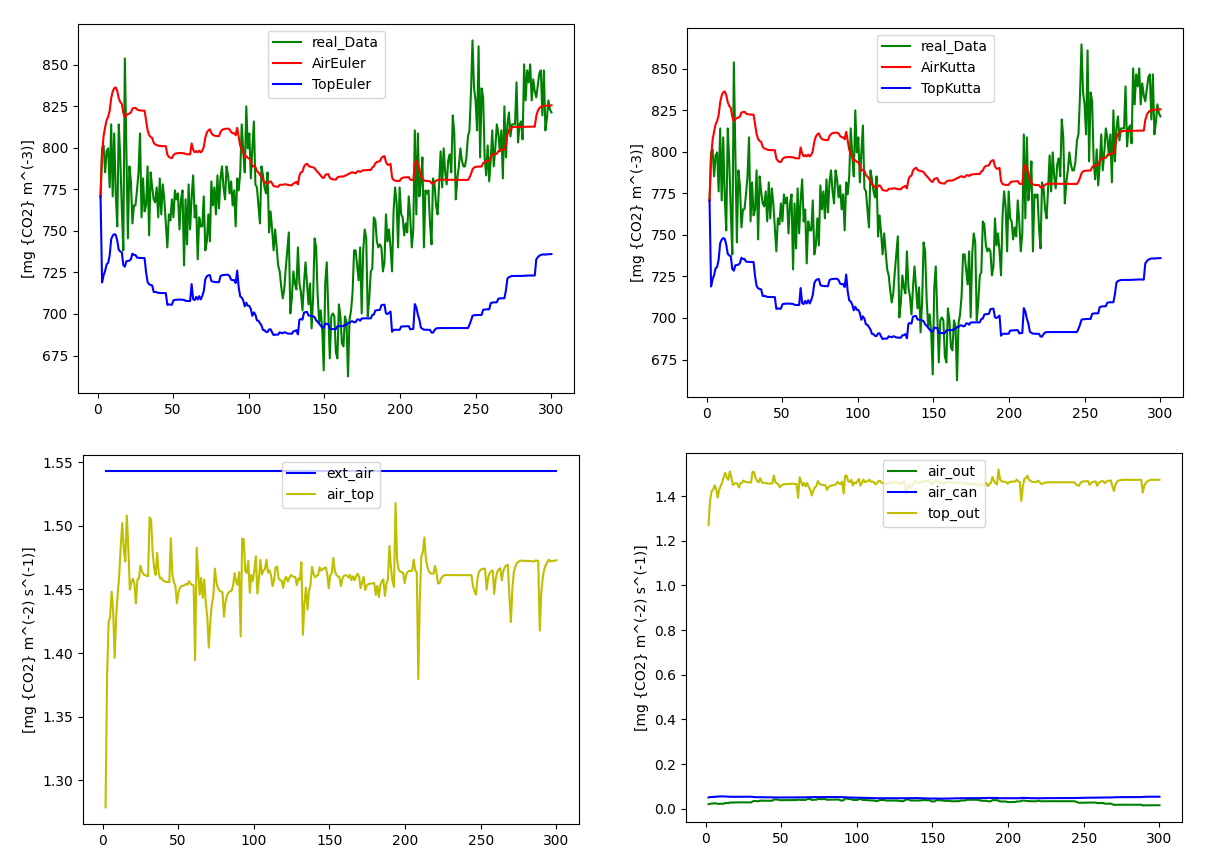
\includegraphics[width=12cm]{sim_co2.png}
				\caption{\textit{Hình ảnh mô phỏng giá trị \co2 trên và dưới màn chắn.}}
				\label{h17}
			\end{center}
		\end{figure} \\
		Dựa vào hình ảnh mô phỏng ở trên, chúng ta có thể rút ra kết luận rằng: Phương pháp tính toán hệ động lực dựa trên hai giải thuật Euler Explicit và Runge Kutta Explicit bậc 4, mặc dù có nhiều thông số được fixed giá trị để giảm bớt độ khó theo yêu cầu đề bài, tuy nhiên kết quả thu được kết quả khá tiệm cận với dữ liệu thật. Do đó, giá trị tính toán được nhìn chung có tính thực tế cao. \\
		Bên cạnh việc chạy dữ liệu mô phỏng, để giá trị tính toán được có tính thực tế hơn cũng như để so sánh với giá trị thực một cách cụ thể, nhóm đã tính toán ra giá trị của $\co2_{Air}$ tại các thời điểm $t+5,t+10,t+15,t+20,t+25$ bằng các sử dụng 2 phương pháp tính toán xấp xỉ Euler và RK4 như được trình bày ở bảng dưới đây:
		\begin{center}
			\begin{tabular}{|c|c|c|c|c|c|}
				\hline
				Thời gian $(t=0)$ & GT thực & Euler & $|\Delta$Euler$|$ & RK4 & $|\Delta|$RK4$|$ \\
				\hline
				$t + 5$ & $799.639$ & $792.6094$ & $7.0296$ & $792.5921$ & $7.0469$ \\
				\hline
				$t + 10$ & $801.444$ & $800.9248$ & $0.5192$ & $800.9099$ & $0.5341$ \\
				\hline
				$t + 15$ & $785.1886$ & $805.1167$ & $19.9281$ & $805.1065$  & $19.9179$ \\
				\hline
				$t + 20$ & $797.8339$ & $810.0681$ & $24.2342$ & $810.0591$ & $24.8705$ \\
				\hline
				$t + 25$ & $799.6389$ & $812.3390$ & $12.7001$ & $812.3329$ & $12.694$ \\
				\hline
			\end{tabular}
		\end{center}
	
	\section{Mô hình hệ động lực đối với áp suất hơi nước trong nhà kính}
		\subsection{Hệ động lực và giả thiết}
			Sự thay đổi áp suất hơi nước ở không gian trên và dưới màn chắn nhiệt trong nhà kính được mô tả bởi hệ phương trình vi phân sau:
			\begin{align}
				\textcolor{blue}{
					cap_{VP_{Air}}\dot{VP_{Air}}} &
				\textcolor{blue}{= MV_{CanAir} + MV_{PadAir} + MV_{FogAir} + MV_{BlowAir}} \nonumber \\
				&\textcolor{blue}{
					 - MV_{AirThScr} - MV_{AirTop} - MV_{AirOut} - MV_{AirOut\_Pad} - MV_{AirMech},} \tag{27} \label{vp1} \\
				\textcolor{blue}{
					cap_{VP_{Top}}\dot{VP_{Top}}} &\textcolor{blue}{= MV_{AirTop} - MV_{TopCov,in} - MV_{TopOut}}
					\tag{28} \label{vp2}
			\end{align}
			Trong đó, $\dot{VP_{Air}}$ và $\dot{VP_{Top}}$ $(kg\ m^{-2}\ s^{-1})$ lần lượt là đạo hàm của áp suất hơi ở gian dưới và trên của màn chắn nhiệt trong nhà kính, $cap_{VP_{Air}}$ và $cap_{VP_{Top}}$ lần lượt là độ ẩm tối đa trong không khí ở gian dưới và trên của màn chắn nhiệt trong nhà kính. \\
			Dưới đây là source code python dùng để hiện thực hệ động lực trên:
\begin{lstlisting}
def derivative(VP_Air, VP_Top, VP_Out):
	CAP_VP_Air = M_water * h_Air / (R * 1000 * T_Air)  # capacity of VP_Air
	CAP_VP_Top = M_water * (h_Gh - h_Air) / (R * 1000 * T_Top)  # capacity of VP_Top
	global temp
	temp -= 1
	mv_air_top = MV_AirTop(VP_Air, VP_Top)
	dVP_Air = (MV_CanAir(VP_Air) + MV_PadAir() + MV_FogAir() + MV_BlowAir() 
			  - MV_AirThScr(VP_Air) - mv_air_top - MV_AirOut(VP_Air, VP_Out)
			  - MV_AirOut_Pad(VP_Air) - MV_AirMech(VP_Air))/CAP_VP_Air
	dVP_Top = (mv_air_top - MV_TopCov_in(VP_Top) - MV_TopOut(VP_Top, VP_Out)) / CAP_VP_Top
	return [dVP_Air, dVP_Top]
\end{lstlisting}
			Hàm \textit{derivative()} trên nhận vào 3 đối số là $VP_{Air}$, $VP_{Top}$ và $VP_{Out}$ tại thời điểm $t$, từ đó hàm sẽ trả về 1 list 2 phần tử là giá trị đạo hàm của $VP_{Air}$ và $VP_{Top}$, từ đó có thể tính được giá trị của chúng tại thời điểm $t+h$.
		\subsection{Các thông số ảnh hưởng tớp áp suất hơi nước}
			Hơi nước trao đổi giữa không khí trong nhà kính và các yếu tố như tán lá ($MV_{CanAir}$), không khí đi ra từ hệ thống thông gió ($MV_{PadAir}$), hệ thống tạo sương ($MV_{FogAir}$), hệ thống làm nóng không khí trực tiếp ($MV_{BlowAir}$), màn chắn nhiệt ($MV_{AirThScr}$), Không khí ngăn trên màn chắn ($MV_{AirTop}$), không khí bên ngoài ($MV_{AirOut}$), lượng không khí ngoài trời qua sự trao đổi của hệ thống thông gió ($MV_{AirOut\_Pad}$) và hệ thống làm mát cơ học ($MC_{AirMech}$), hay hơi nước trao đổi giữa không khí trên màn chắn nhiệt với không khí bên ngoài ($MC_{TopOut}$), với lớp bao bên trong màn chắn nhiệt ($MV_{TopCov,in}$), đều là những yếu tố ảnh hưởng tới tốc độ biến  thiên của áp suất hơi nước và sẽ được mô tả cụ thể sau đây.\\
			Sự thoát hơi nước của lá $MV_{CanAir}$ $(kg\ m^{-2}\ s^{-1})$ được mô tả bởi công thức:
			\begin{align}
				\color{blue}
					MV_{CanAir} = {VEC}_{CanAir}(VP_{Can} - VP_{Air})
				\color{blue}
				\tag{29}\label{vp3}
			\end{align}
			Trong đó, ${VEC}_{CanAir}$ $(Kg\ m^{-2}\ Pa^{-1}\ s^{-1})$ là hệ số trao đổi hơi giữa tán cây và không khí, $VP_{Can}$ $(Pa)$ là áp suất hơi bão hòa tại nhiệt độ tán lá. Hệ số trao đổi hơi giữa tán cây và không khí ${VEC}_{CanAir}$ được mô tả bởi phương trình:
			\begin{align}
				\color{blue}
					VEC_{CanAir} = \dfrac{2\rho_{Air}c_{p,Air}LAI}{\Delta H \gamma (r_b + r_s)}
				\color{blue}
				\tag{30}\label{vp4}
			\end{align}
			Trong đó, $\rho_{Air}$ $(Kg\ m^{-3})$ là mật độ của không khí bên trong nhà kính, $\Delta H$ là nhiệt tiềm ẩn của sự bay hơi của nước, $\gamma$ $(Pa\ K^{-1})$ là hằng số biểu diễn mối liên hệ giữa áp suất riêng phần của nước trong không khí với nhiệt độ không khí, $r_b$ $(m\ s^{-1})$ là sức cản của lớp ngoài của tán lá và $r_s$ $(m\ s^{-1})$ là sức cản của khí khổng trong tán lá tới sự vận chuyển hơi nước. \\
			Sức cản của lớp ngoài của tán lá tới sự vận chuyển hơi nước $r_b$ phụ thuộc vào tốc độ gió trong nhà kính và sự chênh lệch nhiệt độ giữa tán cây và không khí xung quanh. Sức cản của khí khổng trong tán lá tới sự vận chuyển hơi nước $r_s$ được mô tả bằng
			\begin{align}
				\color{blue}
					r_s = r_{s,min}\cdot rf(R_{Can})\cdot rf({CO_2}_{Air\_ppm}) \cdot rf(VP_{Can} - VP_{Air})
				\color{blue}
				\tag{31}\label{vp5}
			\end{align}
			với $r_{s,min}$ là sức cản tối thiểu của tán lá và $rf$ là hệ số cản trong trường hợp mức bức xạ cao, mức \co2 cao và chênh lệch áp suất lớn. Hệ số cản $rf$ được tính bởi các phương trình sau
			\begin{align}
				\textcolor{blue}{
					rf(R_{Can})} &= \textcolor{blue}{\dfrac{R_{Can} + c_{evap1}}{R_{Can} + c_{evap2}}, }
					\tag{32}\label{vp6} \\
					\textcolor{blue}{rf({CO_2}_{Air})} &= \textcolor{blue}{1 + c_{evap3}(\eta_{mg\_ppm} {CO_2}_{Air} - 200)^2} 
					\tag{33}\label{vp7} \\
					\textcolor{blue}{rf(VP_{Can} - VP_{Air})} &= \textcolor{blue}{1 + c_{evap4}(VP_{Can} - VP_{Air})^2}
					\tag{34}\label{vp8}
				\color{blue}
			\end{align}
			trong đó, $R_{Can}$ ${W\ m^{-2}}$ là bức xạ toàn cục trên tán lá, $c_{evap1}$, $c_{evap2}$, $c_{evap3}$ và $c_{evap4}$ là các thông số được xác định từ thực nghiệm, $\eta_{mg\_ppm}$ $(ppm\ m^{3}\ mg^{-1})$ là hệ số chuyển đổi từ $m^{-3}\ mg$ \co2 sang $ppm$. Trên thực tế, các giá trị $c_{evap3}$ và $c_{evap4}$ phụ thuộc vào ngày và đêm. Tuy nhiên, các thông số này có các phương trình đi kèm không thể xác định được tại thời điểm mặt trời mọc và lặn. Để giải quyết vấn đề này, \cite{Sta93} đã đưa ra phương pháp làm mịn tham số $c_{evap3}$ và $c_{evap4}$ bằng công tắc vi sai để các phương trình (\ref{vp6}), (\ref{vp7}), (\ref{vp8}) xác định. Các thông số thoát hơi nước được làm mịn được mô tả bằng:
			\begin{align}
				\textcolor{blue}{
					c_{evap3} = c^{day}_{evap3}(1 - S_{r_s}) + c^{night}_{evap3} S_{r_s}}
					\tag{35}\label{vp9} \\
				\textcolor{blue}{
					c_{evap4} = c^{day}_{evap4}(1 - S_{r_s}) + c^{night}_{evap4} S_{r_s}} 
					\tag{36}\label{vp10}
			\end{align}
			Theo yêu cầu đề bài, vì bị giới hạn về mặt dữ liệu, nên ta sẽ mặc định $r_s = r_{s,min}$. \\
			Qua đó, ta có thể hiện thực hàm tính tốc độ thoát hơi nước của tán lá bằng Python như sau:
\begin{lstlisting}
def saturated(T):
	return -274.36 + 877.52*math.exp(0.0545*(T-273.15))	

def MV_CanAir(VP_Air):
	rs = rs_min*1.1
	# Mat do khong khi duoi man chan nhiet (kg m^{-3})
	p_Air = p_Air0 * math.exp(g * M_Air * h_Elevation / (T_Air * R * 1000))  
	VEC_CanAir = 2*p_Air*c_p_air*LAI/(dentaH*gamma*(rb+rs))
	T_Can = T_Air + 2
	VP_Can = saturated(T_Can)
	can_air = VEC_CanAir*(VP_Can - VP_Air)
	if temp == loop:
		MV_CanAirData.append(can_air)
	return can_air
\end{lstlisting} 
			Hàm \textit{saturated(T)} là hàm sẽ tính giá trị của áp suất hơi bão hòa tại nhiệt độ $T(K)$.Theo yêu cầu đề bài, ta lấy $r_s = r_{s,min}$, tuy nhiên mặc định thì độ chênh lệch so với thực tế là rất lớn, nên nhóm quyết định lấy $r_s = 1.1 \cdot r_{s,min}$ để giá trị xấp xỉ sát với thực nghiệm hơn. Hàm \textit{MV$\_$AirCan} được dùng để tính và trả giá trị của $MV_{CanAir}$ qua việc tính các thành phần liên quan trong phương trình (\ref{vp3}). \\ \\
			
			Tiếp theo, dòng hơi nước đi từ tấm thông gió và hệ thống quạt tới vùng không khí bên trong nhà kính $MV_{PadAir}$  được mô tả bởi phương trình
			\begin{align}
				\color{blue}
					MV_{PadAir} = \rho_{Air}f_{Pad}(\eta_{Pad}(x_{Pad} - x_{Out}) + x_{Out})
				\color{blue}
				\tag{37}\label{vp11}
			\end{align}
			Trong đó, $f_{Pad}$ $(m\ s^{-1})$ là tốc độ hơi nước đi qua bề mặt tấm thông gió và quạt (đã được đề cập trong phương trình (\ref{ct5}))), $\eta_{Pad}$ $(-)$ là độ hiệu quả của hệ thống thông gió và quạt, $x_{Pad}$ và $x_{Air}$ $(Kg\ \{water\}\ Kg^{-1} \{Air^{-1}\})$ lần lượt là hàm lượng hơi nước của tấm thông gió và của không khí bên ngoài.  \\
			Dưới đây là phần hiện thực phương trình (\ref{vp11}):
\begin{lstlisting}
def MV_PadAir():
	# Mat do khong khi duoi man chan nhiet (kg m^{-3})
	p_Air = p_Air0 * math.exp(g * M_Air * h_Elevation/(T_Air * R * 1000))  
	# cuong do khong khi qua tam thong gio (m^3 s^{-1})
	f_Pad = U_Pad * fi_Pad / A_Flr  
	pad_air = p_Air * f_Pad *(eta_pad*(x_pad-x_out) + x_out)
	return pad_air
\end{lstlisting}
			Hàm \textit{MV$\_$PadAir} sẽ hiện thực các tham số thành phần của phương trình (\ref{vp11}), từ đó sẽ tính được giá trị của $MV_{PadAir}$. \\ \\
			
			Ngược lại, dòng hơi nước đi từ vùng không khí bên trong nhà kính đi ra ngoài qua hệ thống thông gió và quạt $MV_{AirOut\_pad}$ được biểu diễn bởi
			\begin{align}
				\color{blue}
					MV_{AirOut\_pad} = f_{Pad}\frac{M_{Water}}{R}(\dfrac{VP_{Air}}{T_{Air} + 273.15})
				\color{blue}
				\tag{38}\label{vp12}
			\end{align}
			trong đó, $M_{Water} = 18$ là khối lượng mol của nước.\\
			Để thể hiện cũng như tính toán giá trị của $MV_{AirOut\_pad}$, ta có thể tham khảo source code dưới đây:
\begin{lstlisting}
def MV_AirOut_Pad(VP_Air):
	f_Pad = U_Pad * fi_Pad / A_Flr # Cuong do khong khi di qua tam khong gio (m^3 s^{-1})
	airOut_pad = f_Pad*M_water/(R*(10**3))*(VP_Air/T_Air)
	return airOut_pad
\end{lstlisting}
			Hàm \textit{MV$\_$AirOut$\_$Pad} sẽ tính toán các giá trị tham số, sau đó trả về kết quả $MV_{AirOut\_pad}$ để hỗ trợ cho việc tính toán hệ đông lực (\ref{vp1})-(\ref{vp1}). \\ \\

			Thông lượng hơi nước từ hệ thống tạo sương đến không khí trong nhà kính $MV_{FogAir}$ được mô tả bởi 
			\begin{align}
				\color{blue}
					MV_{FogAir} = \dfrac{U_{Fog}\phi_{Fog}}{A_{Flr}}
				\color{blue}
				\tag{39}\label{vp13}
			\end{align}
			Trong đó, $U_{Fog}$ $(-)$ là giá trị van điều khiển của hệ thống tạo sương, nhận giá trị trong khoảng $[0,1]$, $\phi_{Fog}$ $(Kg\ \{Water\}\ s^{-1})$ là công suất của hệ thống phun sương.\\
			Dưới đây là source code Python hiện thực tính toán phương trình trên:
\begin{lstlisting}
def MV_FogAir():
	fog_air = U_Fog * fi_Fog / A_Flr
	return fog_air
\end{lstlisting}
			Cụ thể, hàm \textit{MV$\_$FogAir} sẽ dựa vào 3 tham số là $U_{Fog}$, $\phi_{Fog}$ và $A_{Flr}$ để tính toán và trả về giá trị của $MV_{FogAir}$. \\ \\
			
			Cường độ hơi nước từ máy thổi nhiệt đến không khí trong nhà kính $MV_{BlowAir}$ được mô tả tỉ lệ với dòng nhiệt từ máy sưởi không khí đến không khí trong nhà kính $H_{BlowAir}$:
			\begin{align}
				\color{blue}
					MV_{BlowAir} = \eta_{HeatVap}H_{BlowAir}
				\color{blue}
				\tag{40}\label{vp14}
			\end{align}
			Trong đó, $\eta_{HeatVap}$ $(Kg\ {Vapour}\ J^{-1})$ là lượng hơi được giải phóng khi 1 Joule năng lượng được tạo ra bởi máy sưởi không khí. Thông lượng nhiệt $H_{BlowAir}$ được tính bởi:
			\begin{align}
				\color{blue}
					H_{BlowAir} = \dfrac{U_{Blow}P_{Blow}}{A_{Flr}}
				\color{blue}
				\tag{41}\label{vp15}
			\end{align}
			với các thông số được mô tả cụ thể trong phương trình (\ref{ct3}). \\
			Hàm hiện thực phương trình (\ref{vp14}) được mô tả dưới đây:
\begin{lstlisting}
def MV_BlowAir():
	blow_air = (eta_heatVap * U_Blow * P_Blow) / A_Flr
	return blow_air
\end{lstlisting}
			Với giá trị của $H_{BlowAir}$ được thể hiện qua phương trình (\ref{vp15}), kết hợp với phương trình (\ref{vp14}), hàm \textit{MV$\_$BlowAir} sẽ tính được giá trị của $MV_{BlowAir}$ và trả về kết quả tương ứng. \\ \\

			Dựa vào công thức $MV_{12}$ tổng quát, ta có thể biểu diễn thông lượng hơi nước đi từ không khí nhà kính lên màn chắn nhiệt $MV_{AirThScr}$ bằng
			\begin{align}
				\color{blue}
				MV_{AirThScr} = \left\{\begin{array}{llr}
					0,& VP_{Air} < VP_{ThScr} \\
					6.4\cdot 10^{-9} HEC_{AirThScr}(VP_{Air} - VP_{ThScr}), & VP_{Air} > VP_{ThScr}
				\end{array}\right.
				\color{blue}
				\tag{42}\label{vp16}
			\end{align}
			Trong đó, $6.4\cdot 10^{-9}$ là hệ số chuyển đổi từ hệ số trao đổi nhiệt (đơn vị $W\ m^{-2}\ K^{-1}$) thành hệ số trao đổi hơi (Đơn vị $Kg\ m^{-2}\ s^{-1}\ Pa^{-1}$), $HEC_{AirThScr}$ $(W\ m^{-2}\ K^{-1})$ là hệ số trao đổi nhiệt giữ không khí trong nhà kính và trên màn chắn nhiệt. $HEC_{AirThScr}$ được tính bằng 
			\begin{align}
				\color{blue}
					HEC_{AirThScr} = 1.7U_{ThScr}{|T_{Air} - T_{ThScr}|}^{0.33}
				\color{blue}
				\tag{43}\label{vp17}
			\end{align}
			Dưới đây là source code hiện thực phương trình (\ref{vp6})
\begin{lstlisting}
def MV_AirThScr(VP_Air):
	T_ThScr = (T_Air + T_Top) / 2  # Nhiet do cua man chan nhiet
	VP_ThScr = saturated(T_ThScr)
	if (VP_Air < VP_ThScr):
		if temp == loop: 
			MV_AirThScrData.append(0)
		return 0
	
	HEC_AirThScr = 1.7 * U_ThScr * (abs(T_Air - T_ThScr)**0.33)
	air_thScr = 6.4*(10**(-9))*HEC_AirThScr*(VP_Air - VP_ThScr)
	if temp == loop: 
		MV_AirThScrData.append(air_thScr)
	return air_thScr
\end{lstlisting}
			Hàm \textit{MV$\_$AirThScr} sẽ tính các giá trị thành phần của $MV_{AirThScr}$ như $T_{ThScr}$ (Trong phương trình (\ref{vp17})), $HEC_{AirThScr}$ và $VP_{ThScr}$. Với tham số đầu vào là giá trị của $VP_{Air}$ tại thời điểm t, hàm sẽ tính và trả về giá trị của lượng hơi nước trao đổi giữa không gian dưới màn chắn nhiệt và màn chắn nhiệt. \\ \\
			
			Tương tự như vậy, ta có công thức biểu diễn thông lượng hơi nước từ ngăn trên màn chắn nhiệt đến lớp bao bên trong $MV_{TopCov,in}$ là
			\begin{align}
				\color{blue}
				MV_{TopCov,in} = \left\{\begin{array}{llr}
					0,& VP_{Top} < VP_{Cov,in} \\
					6.4\cdot 10^{-9} HEC_{TopCov,in}(VP_{Top} - VP_{Cov,in}).& VP_{Top} > VP_{Cov,in}
				\end{array}\right.
				\color{blue}
				\tag{44}\label{vp18}
			\end{align}
			Với $HEC_{TopCov,in}$ $(W\ m^{-2}\ K^{-1})$ là hệ số trao đổi nhiệt giữ không khí trên màn chắn nhiệt trong nhà kính và lớp bao bên trong, được tính bởi
			\begin{align}
				\color{blue}
				HEC_{TopCov,in} = c_{HECin}{(T_{Top} - T_{Cov,in})}^{0.33}\frac{A_{Cov}}{A_{Flr}}
				\color{blue}
				\tag{45}\label{vp19}
			\end{align}
			Phương trình (\ref{vp18}) sẽ được hiện thực qua hàm dưới đây:
\begin{lstlisting}
'''Calculate MV_TopCov,in'''
def MV_TopCov_in(VP_Top):
	T_Cov_in = (T_Air*2 + T_Top)/3 		# Nhiet do cua lop phu
	VP_Cov_in = saturated(T_Cov_in) 	# ap suat hoi bao hoa cua lop phu
	if VP_Top < VP_Cov_in:
		if temp == loop: 
			MV_TopCov_inData.append(0)
		return 0
	
	HEC_TopCov_in = c_HECin*(abs(T_Top - T_Cov_in)**(0.33))*A_Cov/A_Flr
	top_cov_in = 6.4*(10**(-9))*HEC_TopCov_in*(VP_Top - VP_Cov_in)
	if temp == loop: 
		MV_TopCov_inData.append(top_cov_in)
	return top_cov_in
\end{lstlisting}
			Qua đó, hàm \textit{MV$\_$TopCov$\_$in()} có tham số đầu vào là $VP_{Top}$, hàm tính toán các thông số tương ứng với hai phương trình (\ref{vp18})-(\ref{vp19} sau đó trả về kết quả của $MV_{TopCov,in}$. \\ \\
			
			Dựa trên dạng chung của dòng hơi nước đi từ A đến B được nghiên cứu trong \autocite{Van11}, dòng hơi nước từ không khí dưới màn chắn đến trên màn chắn trong nhà kính $MV_{AirTop}$ được mô tả bởi công thức
			\begin{align}
				\color{blue}
					MV_{AirTop} = \frac{M_{Water}}{R}f_{ThScr}(\dfrac{VP_{Air}}{T_{Air} + 273.15} - \dfrac{VP_{Top}}{T_{Top} + 273.15})
				\color{blue}
				\tag{46}\label{vp20}
			\end{align}
			trong đó, $f_{ThScr}$ là tổng của hai tốc độ gồm tốc độ thẩm thấu qua màn chắn nhiệt và tốc độ tại những nơi không bị chắn bởi màn chắn nhiệt (Đã được mô tả qua phương trình (\ref{ct7})). \\
			Dưới đây là phần hiện thực của phương trình trên:
\begin{lstlisting}
def f_ThScr():
	p_Air = p_Air0 * math.exp(g * M_Air * h_Elevation
			/ (T_Air * R * 1000))
	p_Top = p_Air0 * math.exp(g * M_Air *
	(h_Elevation + h_Air) / (T_Top * R * 1000)) 
	p_MeanAir = p_Air0 * math.exp(g * M_Air *
				(h_Elevation + h_Gh) / ((T_Air + T_Top)/2 * R * 1000))
	
	thScr       = U_ThScr * K_ThScr * (abs(T_Air - T_Top)) ** (2/3)
	notThScr    = (1 - U_ThScr) * ( g*(1 - U_ThScr) / (2*p_MeanAir) 
				* abs(p_Air - p_Top) )**0.5
	return thScr + notThScr
	
def MV_AirTop(VP_Air, VP_Top):
	air_top = M_water/(R*1000)*f_ThScr()*(VP_Air/T_Air - VP_Top/T_Top)
	if temp == loop:
		MV_AirTopData.append(air_top)
	return air_top
\end{lstlisting}
			Với hàm \textit{f$\_$ThScr()} tương tự lấy từ phương trình (\ref{ct7}), hàm \textit{MV$\_$AirTop()} sẽ tính toán và trả về giá trị của cường độ hơi nước đi từ không gian dưới màn chắn nhiệt đến không gian trên màn chắn nhiệt. \\ \\
			
			Tương tự, dòng hơi nước từ không khí trong nhà kính đến không khí bên ngoài $MV_{AirOut}$ được biểu diễn bằng
			\begin{align}
				\color{blue}
					MV_{AirOut} = \frac{M_{Water}}{R}(f_{VentSide} + f_{VentForced})(\dfrac{VP_{Air}}{T_{Air} + 273.15} - \dfrac{VP_{Top}}{T_{Top} + 273.15})
				\color{blue}
				\tag{47}\label{vp21}
			\end{align}
			Trong đó, $f_{VentSide}$ là tốc độ gió của hệ thống quạt trên tường bao xung quanh nhà kính (Đã được mô tả qua phương trình (\ref{ct12})) và $f_{VentForced}$ là tốc độ gió từ hệ thống quạt bên trong nhà kính (Đã được mô tả qua phương trình (\ref{ct13})). \\
			Dưới đây là phần hiện thực của phương trình tính $MV_{AirOut}$:
\begin{lstlisting}
def f_VentRoofSide(A_Roof):
	p1 = (U_Roof*U_Side*A_Roof*A_Side) ** 2
	p2 = (U_Roof * A_Roof) ** 2 + (U_Side * A_Side)**2
	p3 = 2*g*h_Side_Roof*(T_Air - T_Out)/T_Mean
	p4 = ((U_Roof*A_Roof + U_Side*A_Side)/2) ** 2

	if A_Roof == 0 and A_Side == 0: 
		return 0
	return (cd/A_Flr)*( (p1/p2*p3 + p4*cw*(v_wind**2)) ** 0.5 )

# toc do gio cua he thong quat tren tuong
def f_VentSide():
	if U_Roof == 0:
		eta_Roof = 1.1
	else:
		eta_Roof = A_Roof * U_Roof / (A_Side * U_Side + A_Roof * U_Roof)
		eta_Side = (A_Side * U_Side) / (A_Side * U_Side + A_Roof * U_Roof)
	if eta_Roof < eta_Side_Thr:
		return zeta_InsScr() * (U_ThScr * f_VentRoofSide(0) + (1 - U_ThScr)
				* f_VentRoofSide(A_Roof) * eta_Side) + 0.5 * f_Leakage()
	else:
		return zeta_InsScr() * f_VentRoofSide(0) + 0.5 * f_Leakage()

# He so giam do luoi chan con trung
def zeta_InsScr():
	return zeta_Insect * (2 - zeta_Insect)

# Cuong do khong khi ro ri
def f_Leakage():
	if v_wind < 0.25:
		return 0.25*c_leak
	else:
		return v_wind*c_leak

def f_VentForced():
	return zeta_InsScr()*U_VentForced*fi_VentForced/A_Flr

'''Calculate MV_AirOut'''
def MV_AirOut(VP_Air, VP_Out):
	air_out = M_water/(R*1000)*(f_VentSide() + f_VentForced())*(VP_Air/T_Air - VP_Out/T_Out)
	if temp == loop: 
		MV_AirOutData.append(air_out)
	return air_out
\end{lstlisting}	
			Hàm \textit{MV$\_$AirOut()} dựa vào giá trị trả về của các hàm đã được mô tả bởi các phương trình (\ref{ct12})-(\ref{ct13}) để tính toán và trả về giá trị của cường độ hơi nước đi từ gian dưới màn chắn ra ngoài nhà kính. \\ \\
			
			Dòng hơi nước từ không khí trên màn chắn trong nhà kính đến không khí bên ngoài $MV_{TopOut}$ cũng được áp dụng công thức tổng quát trong \cite{Van11}, vì vậy sẽ được mô tả bằng
			\begin{align}
				\color{blue}
					MV_{TopOut} = \frac{M_{Water}}{R}f_{VentRoof}(\dfrac{VP_{Air}}{T_{Air} + 273.15} - \dfrac{VP_{Top}}{T_{Top} + 273.15})
				\color{blue}
				\tag{48}\label{vp22}
			\end{align}
			Trong đó, $f_{VentRoof}$ là tốc độ luồng không khí đi qua ô mở mái nhà kính (Đã được mô tả qua phương trình (\ref{ct15})). \\
			Dưới đây là hàm hiện thực của phương trình (\ref{vp22}):
\begin{lstlisting}
'''Calculate MV_TopOut'''
def MV_TopOut(VP_Top, VP_Out):
	top_out = M_water/(R*1000)*f_VentRoof()*(VP_Top/T_Top - VP_Out/T_Out)
	if temp == loop: 
		MV_TopOutData.append(top_out)
	return top_out

# toc do khong khi di qua o mo mai nha kinh
def f_VentRoof():
	if U_Roof == 0:
		eta_Roof = 1.1
	else:
		eta_Roof = A_Roof * U_Roof / (A_Side * U_Side + A_Roof * U_Roof)
	if eta_Roof < eta_Roof_Thr:
		return zeta_InsScr() * (U_ThScr * f2_VentRoof() + (1 - U_ThScr) 
				* f_VentRoofSide(A_Roof) * eta_Roof) + 0.5 * f_Leakage()
	else:
		return zeta_InsScr() * f2_VentRoof() + 0.5 * f_Leakage()

def f2_VentRoof():
	return (cd*U_Roof*A_Roof)/(2*A_Flr) 
			* ((g*h_Vent*(T_Air-T_Out)/(2*T_Mean)+cw*(v_wind**2) ) ** 0.5)
\end{lstlisting}
			Các hàm \textit{f$\_$VentRoof()} và \textit{f2$\_$VentRoof()} dựa vào giải thuật của phương trình (\ref{ct15}) đã được thể hiện ở phần trước. Dựa vào đó, hàm \textit{MV$\_$TopOut()} sẽ trả về giá trị của cường độ hơi nước đi từ gian trên màn chắn nhiệt ra ngoài nhà kính. \\ \\

			Cuối cùng, thông số ảnh hưởng tới áp suất hơi nước được gồm dòng hơi từ không khí nhà kính đến bề mặt của hệ thống làm mát cơ học, $MV_{AirMech}$. Dựa trên nghiên cứu công thức tổng quát về tốc độ hơi nước từ không khí sang một vật thể trong \cite{Van11},  $MV_{AirMech}$ được biểu diễn bằng
			\begin{align}
				\color{blue}
				MV_{AirMech} = \left\{\begin{array}{llr}
					0,& VP_{Air} < VP_{MechCool} \\
					6.4\cdot 10^{-9} HEC_{MechAir}(VP_{Air} - VP_{MechCool}).& VP_{Air} > VP_{MechCool}
				\end{array}\right.
				\color{blue}
				\tag{49}\label{vp23}
			\end{align}
			Trong đó, $VP_{MechCool}$ $(Pa)$ là áp suất hơi bão hòa của cơ cấu làm mát cơ khí, $HEC_{MechAir}$ $(W\ m^{-2}\ K^{-1})$ là hệ số trao đổi nhiệt giữa không khí bên trong nhà kính với bề mặt của bộ làm mát cơ học, được tính bởi công thức
			\begin{align}
				\color{blue}
					HEC_{AirMech} = \dfrac{U_{MechCool}COP_{MechCool}P_{MechCool}/A_{Flr}}{T_{Air} - T_{MechCool} +6.4\cdot 10^{-9}\Delta H (VP_{Air} - VP_{MechCool})}
				\color{blue}
				\tag{50}\label{vp24}
			\end{align}
			Trong đó, $U_{MechCool}$ $(-)$ là giá trị của van điều khiển của thiết bị làm mát cơ học, giá trị nằm trong khoảng $[0,1]$, $COP_{MechCool}$ $(-)$ là hệ số hiệu suất của hệ thống làm mát cơ học, $P_{MechCool}$ $(W)$ là công suất điện của hệ thống làm mát cơ học và $T_{MechCool}$ $(^oC)$ là nhiệt độ của bề mặt làm mát.
			Ta có thể hiện thực phương trình (\ref{vp23}) bằng Python như sau:
\begin{lstlisting}
'''Calculate MV_AirMech'''
def MV_AirMech(VP_Air):
	T_MechCool = 0
	VP_MechCool = saturated(T_MechCool) 
	
	if VP_Air < VP_MechCool:
		return 0
	numerator = U_MechCool*COP_MechCool*P_MechCool/A_Flr
	denominator = T_Air-T_MechCool + 6.4*(10**(-9))*dentaH*(VP_Air-VP_MechCool)
	HEC_MechAir = numerator/denominator
	
	return 6.4*(10**(-9))*HEC_MechAir*(VP_Air - VP_MechCool)
\end{lstlisting}
	Hàm \textit{MV$\_$AirMech()} sẽ tính toán các giá trị thành phần của phương trình (\ref{vp23}), cụ thể ở đây là tính $HEC_{AirMech}$. Có được các giá trị tham số tương ứng, ta có thể dễ dàng tính được giá trị của $MV_{AirMech}$. Qua đó, hàm sẽ trả về giá trị tương ứng của cường độ hơi nước của gian dưới màn chắn nhiệt bị hút bởi hệ thống làm lạnh.
	
	\subsection{Các tham số của hệ động lực và giải thích}
		Trong source code dùng để hiện thực mô hình hệ động lực thể hiện sự thay đổ của áp suất hơi nước trong nhà kính, có các thông số được xác định bởi \cite{Van11} và được xác định bởi tập dữ liệu lấy từ thực tế. Cụ thể:
\begin{lstlisting}
c_p_air = 1*(10**3)  	# Cong suat nhiet cu the cua khong khi(J.K^{-1}.kg^{-1})
LAI = 2.5  				# Chi so la (m^2 m^{-2})
dentaH = 2.45*(10**6)  	# Nhiet bay hoi an (J.kg^{-1}water)
gamma = 65.8  # (Pa.K^{-1})
rs_min = 82.0  			# Tro khang nho nhat cua la(s.m^{-1})
rb = 275  				# Tro khang cua lop ranh gioi cua la
#------------------------------------------------------------------------------------------
U_Pad = 1       		# Gia tri cua van dieu khien cua tam thong gio
fi_Pad = 0   			# Cong suat khong khi di qua tam thong gio (m^3 s^{-1})
eta_pad = 0  			# Do hieu qua cua he thong thong gio va quat
x_pad = 0  				# thanh phan nuoc cua he thong thong gio (kg water . kg^{-1} air)
x_out = 0  				# thanh phan nuoc cua khong khi ngoai (kg water . kg^{-1} air)
A_Flr = 1.4*(10**4)     
#------------------------------------------------------------------------------------------
U_Fog = 1   			# Van dieu khien cua he thong tao suong
fi_Fog = 0 				# Cong suat hoi nuoc cua he thong tao suong (kg water s^{-1})
#------------------------------------------------------------------------------------------
eta_heatVap = 4.43*(10**(-8))  # Luong hoi nuoc sinh ra khi 1J Q tao ra boi may suoi (kg vapour J^{-1})
U_Blow = 1    			# gia tri van dieu khien cua may suoi
P_Blow = 0     			# Cong suat nhiet cua may suoi khong khi truc tiep (W)
#------------------------------------------------------------------------------------------
U_ThScr = 0.1  			# Gia tri do phu cua man chan nhiet [0,1]
#------------------------------------------------------------------------------------------
g = 9.8                 # Gia toc trong truong (m s^{-2})
M_Air = 28.96           # g mol^{-1}
K_ThScr = 0.05*(10**(-3))    # Kha nang cho khong khi tham thau cua man 
T_Air = 0               # Nhiet do gian tren man chan (K)
T_Top = 0               # nhiet do gian duoi man chan (K) (= T_Air + 1)
h_Elevation = 0         # Do cao cua nha kinh so voi muc nuoc bien (m)
h_Air = 3.8             # Chieu cao cua compartment ben duoi nha kinh (m)
h_Gh = 4.2
p_Air0 = 1.20           # Mat do khong khi o muc nuoc bien (kg m^{3})
#------------------------------------------------------------------------------------------
v_wind = 0     			# Toc do gio
c_leak = 10**(-4)     	# he so ro ri
zeta_Insect = 1   
eta_Roof_Thr = 0.9     	# nguong Stack (o Roof)
eta_Side_Thr = eta_Roof_Thr   # nguong Stack (o Side)
U_ShScr = 0.4 
C_Gh_d = 0.75
C_Gh_w = 0.09
eta_ShScrCd = 0
eta_ShScrCw = 0
cw = C_Gh_w*(1 - eta_ShScrCw*U_ShScr)
cd = C_Gh_d*(1 - eta_ShScrCd*U_ShScr)
U_Side = 1
A_Side = 0*A_Flr
U_Roof = 1
A_Roof = 0.1*A_Flr      # dien tich o thong gio tren mai
eta_Side = (A_Side*U_Side)/(A_Side*U_Side + A_Roof*U_Roof)
h_Side_Roof = 0   # The vertical distance between mid-points of side wall and roof ventilation openings
T_Out = 0    
T_Mean = 0   
U_VentForced = 1 
fi_VentForced = 0  # luu luong khong khi di qua quat gio
#-------------------------------------------------------------------------------------------
M_water = 18   
R = 8.314       
#-------------------------------------------------------------------------------------------
U_MechCool = 1  
COP_MechCool = 0 
P_MechCool = 0  
#-------------------------------------------------------------------------------------------
c_HECin = 1.86  
A_Cov = 1.8*(10**4)  
#-------------------------------------------------------------------------------------------
h_Vent = 0.68                  # the vertical dimension of a single ventilation opening
\end{lstlisting}
		
		\subsection{Các giả định về giá trị}
			Trong Assignment này, nhóm đã đưa ra một vài giả định nhằm khắc phục việc thiếu dữ liệu và để hiện thực bài toán tốt hơn: \\
			$
				T_{Top} = T_{Air} + 5 \\
				T_{Can} = T_{Air} + 2 \\
				r_s = 1.1r_{s,min} \\
				T_Mean = \dfrac{T_{Air} + T_{Top}}{2} \\
				U_{ThScr} = 0.1 \\
				U_{Roof} = \dfrac{VentLee + ventWind}{200}$ \\
				Nếu $U_{Roof} < 0.3$ sẽ tăng $U_{Roof}$ thêm $0.7$ (cho khớp với dữ liệu thực tế hơn) \\
				$T_{ThScr} = \dfrac{T_{Air} + T_{Top}}{2} \\
				T_{Cov,in} = \dfrac{2T_{Air} + T_{Top}}{3}
			$
			
		\subsection{Tính toán xấp xỉ giá trị của áp suất hơi nước trong nhà kính và mô phỏng}
			\subsubsection{Giải thuật tính xấp xỉ hệ động lực}
				Trong phần này, chúng ta vẫn sẽ dùng giải thuật Euler Explicit và Runge Kutta Explicit bậc 4 đã được đề cập ở phần 1 và hiện thực ở phần 3.5.1.
			\subsubsection{Mô phỏng hệ động lực và so sánh với dữ liệu thực}
				Với dữ liệu được lấy từ 2 file \textit{meteo.csv} và \textit{Greenhouse$\_$climate.csv} (2 file này đã được giải thích ở phần 3.5.2), nhóm đã tính toán và trả về giá trị của áp suất hơi nước tại thời điểm $t+h$, sau đó nhóm đã mô phỏng và thu được kết quả của giá trị áp suất hơi nước ở trên và dưới màn chắn nhiệt dựa trên hai giải thuật Euler và Runge Kutta bậc 4 so với dữ liệu thực như sau:
				\begin{figure}[h!]
					\begin{center}
						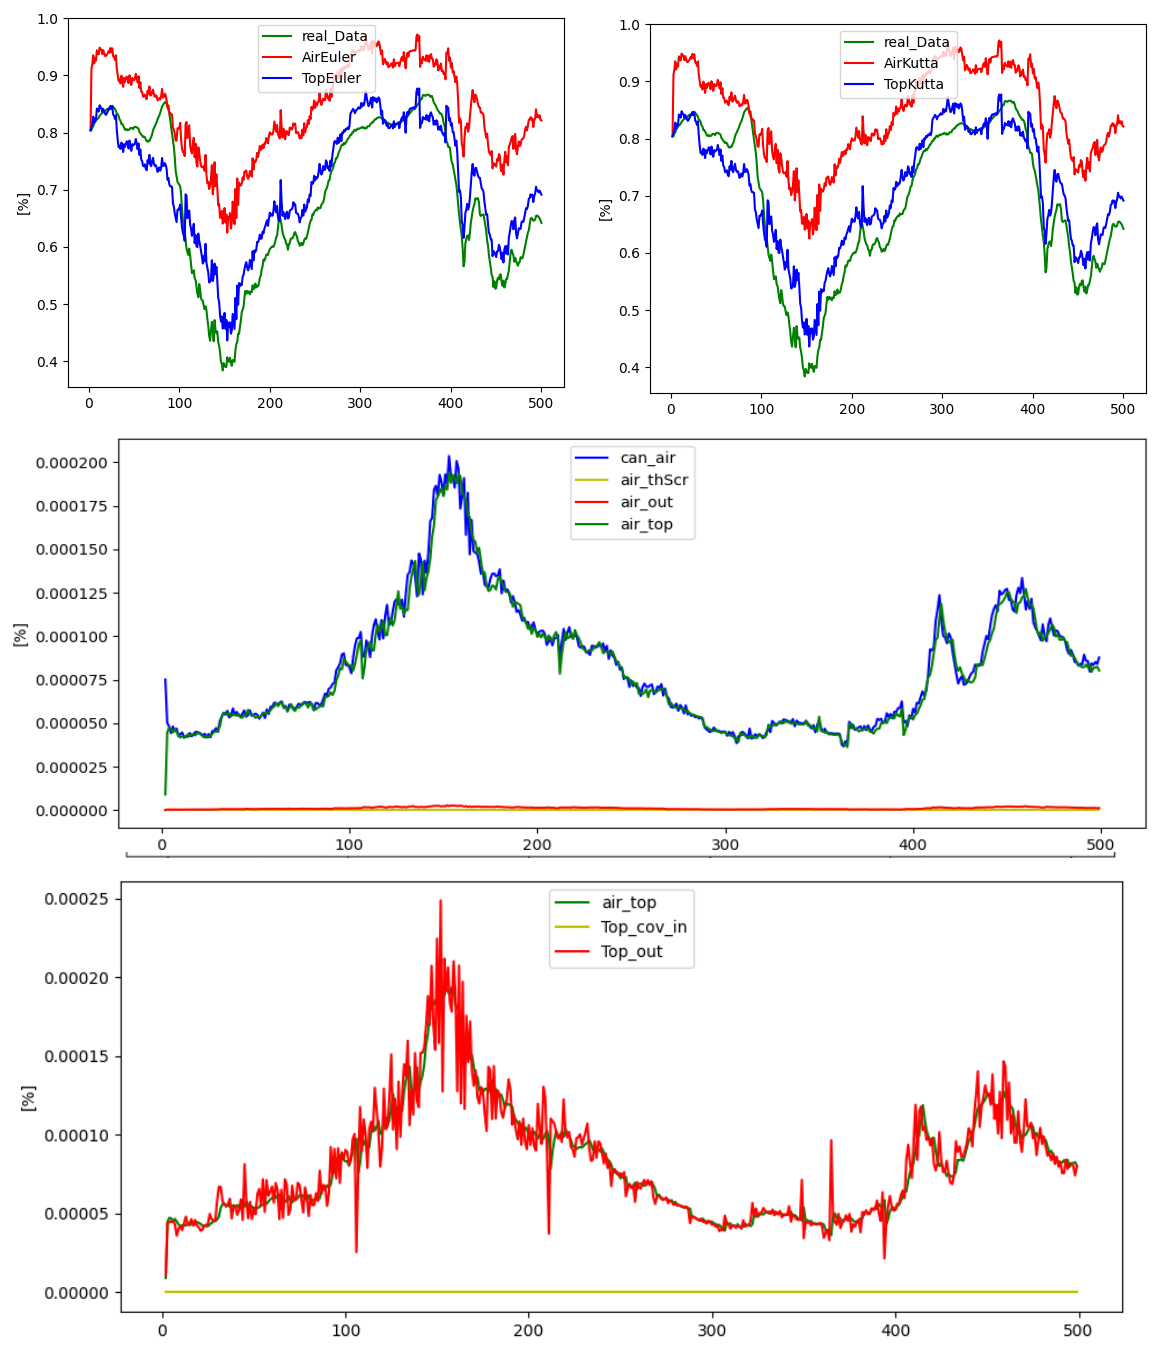
\includegraphics[width=8cm]{sim_h2o.png}
						\caption{\textit{Hình ảnh mô phỏng giá trị của áp suất hơi nước trên và dưới màn chắn.}}
						\label{h18}
					\end{center}
				\end{figure} \\
				Bên cạnh việc chạy dữ liệu mô phỏng, để giá trị tính toán được có tính thực tế hơn cũng như để so sánh với giá trị thực một cách cụ thể, nhóm đã tính toán ra giá trị của $VP_{Air}$ tại các thời điểm $t+5,t+10,t+15,t+20,t+25$ bằng các sử dụng 2 phương pháp tính toán xấp xỉ Euler và RK4 như được trình bày ở bảng dưới đây:
				\begin{center}
					\begin{tabular}{|c|c|c|c|c|c|}
						\hline
						Thời gian $(t=0)$ & GT thực & Euler & $|\Delta$Euler$|$ & RK4 & $|\Delta|$RK4$|$ \\
						\hline
						$t + 5$ & $2321.44$ & $2120.3388$ & $201.1012$ & $2119.8686$ & $201.5714$ \\
						\hline
						$t + 10$ & $2321.44$ & $2141.7843$ & $179.6557$ & $2141.7062$ & $179.7338$ \\
						\hline
						$t + 15$ & $2293.3$ & $2148.9042$ & $144.3958$ & $2148.8841$  & $144.4159$ \\
						\hline
						$t + 20$ & $2321.44$ & $2141.5689$ & $179.8771$ & $2141.5806$ & $179.8594$ \\
						\hline
						$t + 25$ & $2307.33$ & $2151.8117$ & $155.5183$ & $2151.8117$ & $155.5123$ \\
						\hline
					\end{tabular}
				\end{center}
				Dựa vào hình ảnh mô phỏng ở trên, chúng ta có thể rút ra kết luận rằng: Phương pháp tính toán hệ động lực dựa trên hai giải thuật Euler Explicit và Runge Kutta Explicit bậc 4 thu được kết quả khá tiệm cận với dữ liệu thật, tuy nhiên có hơi lệch vì trong quá trình tính toán, có những tham số được fixed vì có những giá trị không đủ dữ liệu để xác định, ví dụ như giá trị $r_s = r_{s,min}$ được fixed so với $r_s$ được phân tích trong \cite{Van11}. \\
	\newpage
	\begin{thebibliography}{80}
		\bibitem[Bal89]{Bal89}	LJ Balemans. Assessment of criteria for energetic effectiveness of greenhouse screens. 1989.
		
		\bibitem[MG]{MG} N.J.van de Braak MIGUEL A.F. and 1995 G.P.ABot. \textit{``Mass flow through materials with pores and openings: II-natural convection''}. In: \textit{submitted for publication in International Journal of Heat and Mass Transfer ()}.
			
		\bibitem[Sta93]{Sta93} C. Stanghellini and J.A. Bunce. \textit{Response of photosynthesis and conductance to light, CO2, temperature and humidity in tomato plants grown at ambient and elevated CO2}. 1993.
		
		\bibitem[Van11]{Van11}
		Bram HE Vanthoor. \textit{A model-based greenhouse design method}. 2011.
		
		\bibitem[De96]{De96}
		HF De Zwart. \textit{Analyzing energy-saving options in greenhouse cultivation using a simulation model}. 1996.

		%\clearpage
		\addcontentsline{toc}{section}{Tài liệu tham khảo}
		\printbibliography
	\end{thebibliography}
\end{document}